\documentclass[conference]{IEEEtran}

\usepackage[utf8]{inputenc}
\usepackage[T1]{fontenc}
\usepackage{amsmath,amssymb}
\usepackage{graphicx}
\usepackage{booktabs}
\usepackage{multirow}
\usepackage{array}
\usepackage{algorithm}
\usepackage{algpseudocode}
\usepackage[numbers,square,sort&compress]{natbib}
\usepackage{hyperref}
\usepackage{xcolor}
\usepackage{caption}

\hypersetup{
    colorlinks=true,
    linkcolor=blue,
    citecolor=blue,
    urlcolor=blue
}

\begin{document}

\title{A Surrogate-Assisted Genetic Algorithm for the Capacitated Facility\\
Location Problem: Extending Linear Programming--Genetic Algorithm\\
Hybridisation with a Machine Learning Fitness Surrogate}

\author{
\IEEEauthorblockN{Yasaswini Chebolu}
\IEEEauthorblockA{Department of Computer Science and Engineering (AI \& ML)\\
Gayatri Vidya Parishad College of Engineering for Women}
}

\maketitle

\begin{abstract}
The Capacitated Facility Location Problem (CFLP) couples a binary decision of
which facilities to open with a continuous transportation-allocation
sub-problem. A well-established strategy, previously demonstrated by Ozsoydan
and G\"{o}lc\"{u}k (2023), decomposes CFLP into a binary sub-problem solved by
an evolutionary/swarm-based search and a continuous transportation sub-problem
solved exactly by a linear programming (LP) solver. This paper studies a
further hybridisation of the same decomposition: replacing the exact LP
fitness evaluation inside the evolutionary loop with a trained machine
learning (ML) surrogate model, invoking the exact solver only when a
surrogate prediction indicates a new best-known solution. We describe a
bootstrap mechanism that trains the surrogate directly from a genetic
algorithm's (GA) own search trajectory, removing the need for a pre-existing
training corpus, and a confidence-aware evaluation policy governing when
exact re-verification is triggered. The proposed Hybrid ML-GA framework and a
classical GA baseline are benchmarked on all 40 standard Beasley OR-Library
CFLP instances (cap41--cap134, capa--capc). The surrogate-assisted approach
recovers the published optimum in its best run on every instance up to 25
facilities, but Wilcoxon signed-rank tests on 400 matched paired runs show the
classical GA to be significantly better in every instance-size group -- a
difference that is practically negligible on the small and medium instances
(mean gaps of 0.055\% versus 0.125\%) yet large on the three 100-facility
instances (10.4\% versus 19.6\%). Three further experiments sharpen the
picture. First, an active-learning extension that grows the training corpus
roughly tenfold and improves surrogate $R^2$ on all three large instances
nonetheless \emph{worsens} the optimality gap on two of them, contradicting
the intuitive hypothesis that the large-instance deficit is simply a
sampling-budget problem. Second, a comparison of four surrogate architectures
shows that $R^2$ is a misleading accuracy metric in this setting -- a Random
Forest attains $R^2 = 0.998$ while its MAPE on the same predictions exceeds
$500{,}000\%$, because Big-M capacity penalties dominate the variance that
$R^2$ normalises against. Third, and most consequentially, substituting the
markedly more accurate Gradient Boosting surrogate (bounded worst-case MAPE of
5.5\% against the Random Forest's 948{,}600\%) under an otherwise identical
protocol changes solution quality negligibly and insignificantly
($p = 0.33$), producing \emph{bit-identical} results on 33 of the 40
instances. Together these two negative results expose a structural property of
the confidence-aware policy: because the incumbent is updated only after exact
verification, the surrogate can discard good candidates but never contribute a
solution, so its accuracy is decoupled from the quality of what the search
returns. Robustness of individual-based model management above an accuracy
threshold is known in the surrogate-assisted evolutionary algorithm literature;
what these results add is that mandatory verification makes the decoupling
exact rather than statistical, and makes it hold even for a surrogate far below
any such threshold. The surrogate's contribution is thus computational rather
than qualitative, which explains why improving it does not help and indicates
what a solution-quality-improving design would have to change. Full per-run
statistics are
reported for every instance rather than only best-run gaps, and two
implementation defects found during verification -- a data-corruption bug in
the OR-Library template parser and a thread-safety crash in the classical GA's
large-instance fitness evaluator -- are documented alongside the results they
affected.
\end{abstract}

\begin{IEEEkeywords}
Capacitated facility location problem, genetic algorithm, machine learning
surrogate model, linear programming hybridisation, surrogate-assisted
optimisation, supply chain network design
\end{IEEEkeywords}

\section{Introduction}

Facility location decisions determine the long-run cost structure of a supply
chain: where to build or lease warehouses, how much capacity to commit, and
how to route customer demand to the opened facilities. The Capacitated
Facility Location Problem (CFLP) formalises this decision as the joint choice
of a binary facility-opening vector and a continuous transportation-allocation
policy that together minimise the sum of fixed opening costs and variable
transportation costs, subject to per-facility capacity limits and full demand
satisfaction \citep{beasley1988,contreras2010}. CFLP is NP-hard, and exact
methods based on mixed-integer linear programming (MILP), Lagrangean
relaxation, and Benders decomposition become computationally expensive as the
number of candidate facilities grows \citep{fischetti2016,vanroy1986}.

A recurring and effective idea in the CFLP literature is problem decomposition:
once the binary facility-opening decisions are fixed, the remaining
transportation-allocation problem is a continuous linear program solvable to
optimality in polynomial time. Ozsoydan and G\"{o}lc\"{u}k \citep{ozsoydan2023}
formalise this idea by decomposing CFLP into a binary sub-problem $P_1$,
solved by a swarm-intelligence-inspired evolutionary algorithm (denoted mSI)
using genetic-algorithm-style crossover and an adaptive mutation operator, and
a continuous sub-problem $P_2$, solved exactly by a linear solver for every
binary vector the search generates. Their study, which forms the basis of the
present work, avoids the transfer (sigmoid) functions typically used to map
continuous swarm-intelligence updates onto binary domains, and reports
statistically verified, near-optimal results across the full Beasley
OR-Library CFLP benchmark suite.

The present study adopts the same $P_1$/$P_2$ decomposition and the same
benchmark suite, but investigates a complementary hybridisation direction not
explored in \citep{ozsoydan2023}: rather than hybridising an evolutionary
algorithm with an exact solver only, we additionally hybridise it with a
\emph{machine learning surrogate} that approximates the outcome of the exact
LP sub-problem. The motivation is computational: solving the transportation LP
exactly for every individual in every generation is the dominant cost of the
GA's inner loop, particularly as instance size grows. If a sufficiently
accurate surrogate can predict the cost of a candidate facility configuration
in microseconds rather than milliseconds, the exact solver can be reserved
for the comparatively rare candidates that appear genuinely promising, while
the bulk of the population is still steered by a reasonably accurate signal.

This paper makes the following contributions:
\begin{enumerate}
    \item A \textbf{bootstrap mechanism} resolving the circular dependency
    between needing a trained surrogate to run the hybrid GA and needing a GA
    run to generate the surrogate's training data: the hybrid solver can be
    run with no surrogate at all, in which case it behaves as a classical
    exact-LP GA while logging every evaluated (chromosome, cost) pair as
    training data for the surrogate's first iteration.
    \item A \textbf{confidence-aware decision rule} for when to trust the
    surrogate versus invoke the exact solver: the exact LP sub-problem is
    solved only when the surrogate's predicted cost is lower than the best
    cost found so far in the run.
    \item A \textbf{full re-benchmark on all 40 OR-Library CFLP instances},
    reporting not only best-run gaps but the complete per-instance statistics
    (best, average, worst, median, standard deviation) for both solvers, plus
    Wilcoxon signed-rank tests over 400 matched paired runs establishing where
    the observed differences are statistically significant and, separately,
    where they are practically consequential.
    \item An \textbf{experimental refutation of the intuitive explanation} for
    the framework's large-instance deficit: an active-learning extension that
    enlarges the training corpus roughly tenfold and improves surrogate $R^2$
    on all three 100-facility instances nevertheless worsens the optimality
    gap on two of them, showing that the deficit is not simply a
    sampling-budget problem.
    \item A \textbf{methodological caution about $R^2$} for surrogate-assisted
    combinatorial optimisation, together with a four-way architecture
    comparison: where Big-M constraint penalties enter the training corpus
    they dominate the variance $R^2$ normalises against, so a model can score
    $R^2 = 0.998$ while being wrong by a factor of thousands on the
    ordinary-cost solutions that actually guide the search.
    \item An \textbf{exact demonstration, on a real combinatorial problem, of
    the decoupling between surrogate accuracy and solution quality} under
    verification-gated model management. Substituting a surrogate five orders
    of magnitude more accurate in worst-case MAPE leaves solutions
    bit-identical on 33 of 40 instances, because a policy that updates the
    incumbent only after exact verification allows the surrogate to discard
    good candidates but never to contribute one. Robustness of individual-based
    model management above an accuracy threshold is already established
    \citep{hanawa2025}; the contribution here is that mandatory verification
    makes the decoupling exact rather than statistical, and makes it hold even
    for a catastrophically inaccurate surrogate far below any such threshold.
    This single mechanism accounts for both negative results above and
    delimits what surrogate-assisted CFLP search of this form can deliver.
    \item A \textbf{documented account of implementation defects} discovered
    during verification -- a silent data-corruption bug in the OR-Library
    template parser and a thread-safety native crash in the classical GA's
    large-instance evaluator -- together with their fixes, so the reported
    results are reproducible and the audit trail is preserved.
\end{enumerate}

The remainder of the paper is organised as follows. Section~II presents the
CFLP formulation and reviews closely related literature. Section~III
describes the proposed Hybrid ML-GA framework. Section~IV reports the
computational study across all 40 OR-Library instances, covering full run
statistics, convergence behaviour, the surrogate architecture comparison, and
the significance tests. Section~V discusses the large-instance limitation,
reports the active-learning experiment that tests the leading explanation for
it, and documents the defects found and corrected during verification.
Section~VI concludes.

\section{Problem Formulation and Related Literature}

\subsection{Formulation of CFLP}

Let $I$ denote the set of $m$ candidate facility locations and $J$ the set of
$n$ customers. Each facility $i \in I$ has a fixed opening cost $f_i$ and a
capacity $s_i$; each customer $j \in J$ has a demand $d_j$. Let $c_{ij}$
denote the transportation cost associated with facility $i$ serving customer
$j$'s full demand. Let $y_i \in \{0,1\}$ indicate whether facility $i$ is
opened, and let $x_{ij} \ge 0$ denote the fraction of customer $j$'s demand
served by facility $i$. The problem is

\begin{align}
\min \quad & Z = \sum_{i \in I} f_i y_i + \sum_{i \in I} \sum_{j \in J} c_{ij}\, x_{ij}\, d_j
\label{eq:obj} \\
\text{s.t.} \quad
& \sum_{i \in I} x_{ij} = 1 && \forall j \in J \label{eq:demand} \\
& x_{ij} \le y_i && \forall i \in I,\, j \in J \label{eq:link} \\
& \sum_{j \in J} d_j\, x_{ij} \le s_i\, y_i && \forall i \in I \label{eq:capacity} \\
& x_{ij} \ge 0, \quad y_i \in \{0,1\} && \forall i \in I,\, j \in J \label{eq:domain}
\end{align}

Eq.~\eqref{eq:demand} ensures every customer's demand is fully allocated;
Eq.~\eqref{eq:link} permits allocation only to opened facilities;
Eq.~\eqref{eq:capacity} enforces facility capacity limits. This follows the
Beasley OR-Library convention, in which $c_{ij}$ is the flat total cost of
fully serving customer $j$'s entire demand from facility $i$ (not a per-unit
rate); this convention is applied consistently across every cost computation
in the implementation and verified against the published optimal cost of
\emph{cap71} (\$932{,}615.75). Fixing $y$ reduces the remaining problem to a
classical transportation problem, solvable in polynomial time -- the property
exploited by the decomposition strategy adopted throughout this paper.

\subsection{Related Literature}

CFLP has an extensive exact-methods literature, including Lagrangean
relaxation \citep{christofides1983,beasley1988}, Benders decomposition
\citep{vanroy1986,wentges1996}, and branch-and-price / branch-and-cut methods
\citep{klose2007,fischetti2016}. Metaheuristic approaches include Tabu Search
\citep{sun2012}, Kernel Search \citep{guastaroba2012}, and RAMP
\citep{matos2021}. Several studies hybridise evolutionary or swarm-based
metaheuristics with exact linear solvers for the transportation sub-problem
specifically: Rahmani and MirHassani \citep{rahmani2014} hybridise a Firefly
Algorithm with a GA under the same $P_1$/$P_2$ decomposition used here, and
Ozsoydan and G\"{o}lc\"{u}k \citep{ozsoydan2023} -- the base study for the
present work -- propose a PSO-inspired evolutionary algorithm (mSI) with an
adaptive, exponentially decreasing bit-flip mutation rate, outperforming
Particle Swarm Optimization and the Grey Wolf Optimizer under matched
conditions. None of the CFLP studies cited above replace the exact
transportation-LP evaluation with a learned approximation; the LP solver is
always invoked for every candidate solution the metaheuristic generates.

Surrogate-assisted metaheuristics have, however, already been applied to
facility location problems, and this study does not claim priority for the
idea. Guo et al.\ \citep{guo2017} solve the two-stage CFLP with a hybrid
evolutionary algorithm in which an extreme learning machine approximates the
fitness of most individuals -- the closest antecedent to the present work.
More recently, surrogate-assisted metaheuristics have been developed for
facility location with demand distributed along network edges
\citep{turkes2024}, including a multi-surrogate differential evolution that
compares random forest, extreme learning machine and gradient-boosting
surrogates \citep{multisurrogate2024}. Wang et al.\ \citep{ecopsurvey2024}
survey the broader field of surrogate-assisted evolutionary algorithms for
expensive combinatorial optimisation. Relative to this literature, the
distinguishing features of the present study are its use of the $P_1$/$P_2$
decomposition with an exact LP sub-solver as the ground-truth evaluator, a
surrogate bootstrapped from the GA's own trajectory rather than from a
pre-existing design of experiments, and -- principally -- its focus on what the
verification gate implies for the relationship between surrogate accuracy and
solution quality, rather than on proposing a faster solver.

Machine-learning surrogate fitness functions are, however, well established in
expensive optimisation more broadly, where the field of surrogate-assisted
evolutionary algorithms (SAEAs) has developed a mature vocabulary for the
question this paper ultimately confronts. Jin \citep{jin2011} distinguishes
several \emph{model management} (or \emph{evolution control}) strategies
governing when the exact evaluator is invoked in preference to the surrogate:
\emph{generation-based} control evaluates entire generations exactly at
intervals; \emph{individual-based} control selects particular individuals for
exact evaluation by some criterion; and \emph{pre-selection} uses the surrogate
to screen candidates before exact evaluation. The confidence-aware policy
studied here (Section~III-E) is an individual-based strategy whose selection
criterion is predicted improvement over the incumbent, coupled with mandatory
exact verification before the incumbent may be updated.

That framing matters for interpreting this paper's results. Hanawa et al.\
\citep{hanawa2025}, using a pseudo-surrogate of tunable accuracy on standard
continuous benchmarks, report that pre-selection improves steadily with
surrogate accuracy whereas individual-based and generation-based control
``exhibit robust performance when the accuracy surpasses a certain
threshold'' -- that is, beyond some accuracy level, further improving the
surrogate stops improving the search. The decoupling reported in
Section~IV-H is consistent with that finding and should be read as confirming
and sharpening it rather than as discovering it. What this study adds is
threefold: the effect is demonstrated on a real constrained combinatorial
problem with genuinely trained surrogates rather than on synthetic benchmarks
with a pseudo-surrogate; the decoupling proves not merely statistical but
\emph{exact}, with bit-identical solutions on 33 of 40 instances; and it
persists even when the surrogate is catastrophically inaccurate (a MAPE of
$521{,}100\%$ on \emph{cap41}, far below any plausible accuracy threshold),
which the mandatory-verification design explains and which a threshold account
alone does not predict.

Random Forests provide a convenient uncertainty estimate via inter-tree
prediction variance \citep{breiman2001}, which motivates their use as the
default surrogate here. The present study combines the $P_1$/$P_2$ CFLP
decomposition of \citep{ozsoydan2023,rahmani2014} with a bootstrap-trained ML
surrogate that replaces the majority of exact LP evaluations inside the
evolutionary loop, while retaining a confidence-gated fallback to the exact
solver.

\section{Proposed Solution Approach}

\subsection{Overview}

A candidate solution is represented as a binary chromosome $y \in \{0,1\}^m$
denoting which facilities are open. Two evaluation strategies for this
chromosome are studied: a \textbf{classical GA} baseline, in which every
chromosome is evaluated by solving the exact transportation LP, and the
\textbf{Hybrid ML-GA}, in which chromosomes are evaluated primarily by a
trained ML surrogate, with the exact LP solver invoked selectively. Both
solvers use the same DEAP-based \citep{fortin2012} evolutionary operators --
tournament selection, two-point crossover, and per-bit mutation -- and the
same generational loop, so that any difference in final solution quality can
be attributed to the fitness evaluation strategy rather than to the search
operators.

\subsection{Classical GA and Exact Fitness Evaluation}

For a chromosome $y$, exact fitness evaluation proceeds in three stages of
increasing computational cost: (1) a feasibility check that penalises $y$
heavily if total open capacity is below total demand; (2) an uncapacitated
shortcut that assigns each customer to its cheapest open facility and returns
this cost directly if no capacity constraint is violated; and (3), otherwise,
an exact transportation LP solved via SciPy's HiGHS backend. Early
convergence detection terminates a run once 10 consecutive generations each
improve the best-found cost by less than $0.01\%$.

\subsection{Feature Representation and Surrogate Model}

Each chromosome is transformed into an engineered feature vector before being
passed to the surrogate: the number of open facilities, capacity utilisation
ratios, cost-weighted facility indicators, and similarity measures relative to
the best chromosomes seen so far. The surrogate is a Random Forest regressor
(200 trees, maximum depth 15, minimum leaf size 1, $\sqrt{\text{features}}$
per split), chosen because inter-tree prediction variance provides a
model-native uncertainty estimate \citep{breiman2001}.

\subsection{Bootstrap Mechanism}

A trained surrogate requires labelled (chromosome, exact-cost) pairs, but
producing enough of them otherwise implies running an exact-LP GA first --
precisely what the surrogate is meant to accelerate. The proposed framework
resolves this by allowing the Hybrid ML-GA solver to be instantiated with no
surrogate at all. In this mode it behaves identically to the classical GA,
but every evaluated (chromosome, cost) pair is logged; after deduplication,
these pairs form the surrogate's initial training corpus. This converts a
cold-start problem into a single pipeline: bootstrap $\rightarrow$ train
$\rightarrow$ solve.

\subsection{Confidence-Aware Evaluation Policy}

The surrogate predicts a cost $\hat{c}$ for every chromosome. If
$\hat{c} \ge c^{\ast}$, where $c^{\ast}$ is the best exact cost found so far,
the prediction is trusted directly. If $\hat{c} < c^{\ast}$ -- the surrogate
claims a new best solution -- the exact LP solver verifies the true cost
before the chromosome updates $c^{\ast}$ or the elite set. Algorithm~1
summarises this policy. A warm-up fraction of the earliest generations
(15--20\% of total generations) always uses exact evaluation, so the elite
set the rule compares against is already well-verified before the surrogate
is trusted.

\begin{algorithm}[t]
\caption{Confidence-aware fitness evaluation for chromosome $y$}
\begin{algorithmic}[1]
\Require chromosome $y$, surrogate $S$, best-so-far cost $c^{\ast}$, generation $t$, warm-up generations $t_w$
\If{$t \le t_w$ \textbf{or} $S$ is unavailable}
    \State $c \gets \textsc{ExactEvaluate}(y)$
\Else
    \State $\hat{c} \gets S.\textsc{Predict}(\textsc{Features}(y))$
    \If{$\hat{c} < c^{\ast}$}
        \State $c \gets \textsc{ExactEvaluate}(y)$
        \If{$c < c^{\ast}$} \State $c^{\ast} \gets c$ \EndIf
    \Else
        \State $c \gets \hat{c}$
    \EndIf
\EndIf
\State \Return $c$
\end{algorithmic}
\end{algorithm}

\subsection{Optional Active Learning}

A quality-gated active-learning extension is also implemented: successive
runs contribute newly observed exact evaluations back into the training
corpus, and the surrogate is retrained after each round, but a retrained
surrogate is only \emph{adopted} if it performs at least as well as the best
model observed across all earlier rounds on a fixed validation set. The
validation set is carved once from the initial bootstrap corpus and held
unchanged thereafter, so that $R^2$ remains comparable across rounds; as
Section~V-B shows, this design choice has a consequence that is not obvious in
advance. This mechanism is not used for the headline results of
Section~IV; it is evaluated separately in Section~V-B as a test of the leading
explanation for the large-instance gap.

\section{Computational Study}

\subsection{Benchmark Suite and Experimental Setup}

All 40 Beasley OR-Library CFLP instances are used: 25 small/medium instances
(\emph{cap41--cap104}, 16 or 25 facilities $\times$ 50 customers), 12 large
instances (\emph{cap111--cap134}, 50 facilities $\times$ 50 customers), and 3
extremely large instances (\emph{capa4}, \emph{capb4}, \emph{capc4}, 100
facilities $\times$ 1000 customers). Published optimal costs are used as
ground truth for all optimality gaps. The classical GA uses population 120 /
100 generations / 30 runs for small/medium instances and population 40 / 60
generations / 10 runs for the 3 large instances (a reduced budget necessitated
by a defect discussed in Section~V-B). The Hybrid ML-GA bootstraps with
population 30 / 15 generations (small/medium) or 60 / 40 generations (large),
trains a Random Forest surrogate on the deduplicated corpus, then solves with
population 120 / 100 generations across 10 confidence-aware runs (warm-up
fraction 0.15). All seeds derive deterministically from a fixed base seed.

\subsection{Full Run Statistics: Classical GA}

Table~\ref{tab:full_classical} reports the complete per-run statistics for the
classical GA -- best, average, worst, and standard deviation of cost, plus
best- and average-run gaps -- rather than only the best-run gap. This is
included specifically because the best-run gap alone is $0.00\%$ for most
small/medium instances (the GA reliably rediscovers the published optimum in
at least one of its 30 runs), which can look uninformative in isolation; the
standard deviation and worst-run columns show that individual runs do vary
substantially, particularly as instance size grows.

\begin{table}[t]
\centering
\caption{Classical GA: full per-run statistics (representative instances across all four size groups). Std.\ Dev.\ and Worst columns show that individual runs vary even where the Best-Gap column is 0.00\%.}
\label{tab:full_classical}
\resizebox{\columnwidth}{!}{
\begin{tabular}{lrrrrr}
\toprule
Instance & Best Cost & Worst Cost & Std.\ Dev. & Best Gap (\%) & Avg Gap (\%) \\
\midrule
cap41  & 1{,}040{,}444 & 1{,}040{,}444 & 0.0 & 0.0000 & 0.0000 \\
cap51  & 1{,}025{,}208 & 1{,}027{,}374 & 487.5 & 0.0000 & 0.0214 \\
cap63  & 1{,}014{,}062 & 1{,}015{,}650 & 476.1 & 0.0000 & 0.0158 \\
cap83  & 975{,}890 & 984{,}179 & 2{,}636.9 & 0.0000 & 0.2606 \\
cap91  & 796{,}648 & 800{,}005 & 774.9 & 0.0000 & 0.0533 \\
cap111 & 826{,}125 & 835{,}181 & 2{,}559.1 & 0.0000 & 0.4242 \\
cap113 & 971{,}377 & 993{,}280 & 5{,}358.2 & 0.0834 & 0.7436 \\
cap114 & 1{,}066{,}135 & 1{,}089{,}993 & 6{,}631.9 & 0.2613 & 1.2693 \\
cap131 & 793{,}440 & 801{,}150 & 2{,}263.0 & 0.0000 & 0.4286 \\
capa4  & 17{,}480{,}386 & 20{,}968{,}663 & 1{,}117{,}476 & 1.8634 & 13.2337 \\
capb4  & 13{,}696{,}499 & 14{,}740{,}241 & 353{,}432 & 4.6877 & 8.7925 \\
capc4  & 11{,}929{,}944 & 13{,}124{,}485 & 365{,}897 & 3.6858 & 9.0996 \\
\bottomrule
\end{tabular}}
\end{table}

The pattern is consistent across every instance: as facility count grows from
16 (\emph{cap41}) to 100 (\emph{capa4}/\emph{capb4}/\emph{capc4}), the standard
deviation of the 30-run cost distribution grows by roughly three orders of
magnitude (from $0$ to over \$1{,}100{,}000), even though the best-run gap
only grows from $0.00\%$ to $1.86$--$4.69\%$. Reporting only the best-run gap
would understate how much harder the search problem becomes at scale; Fig.~1
visualises this trend across all 40 instances.

\begin{figure}[t]
\centering
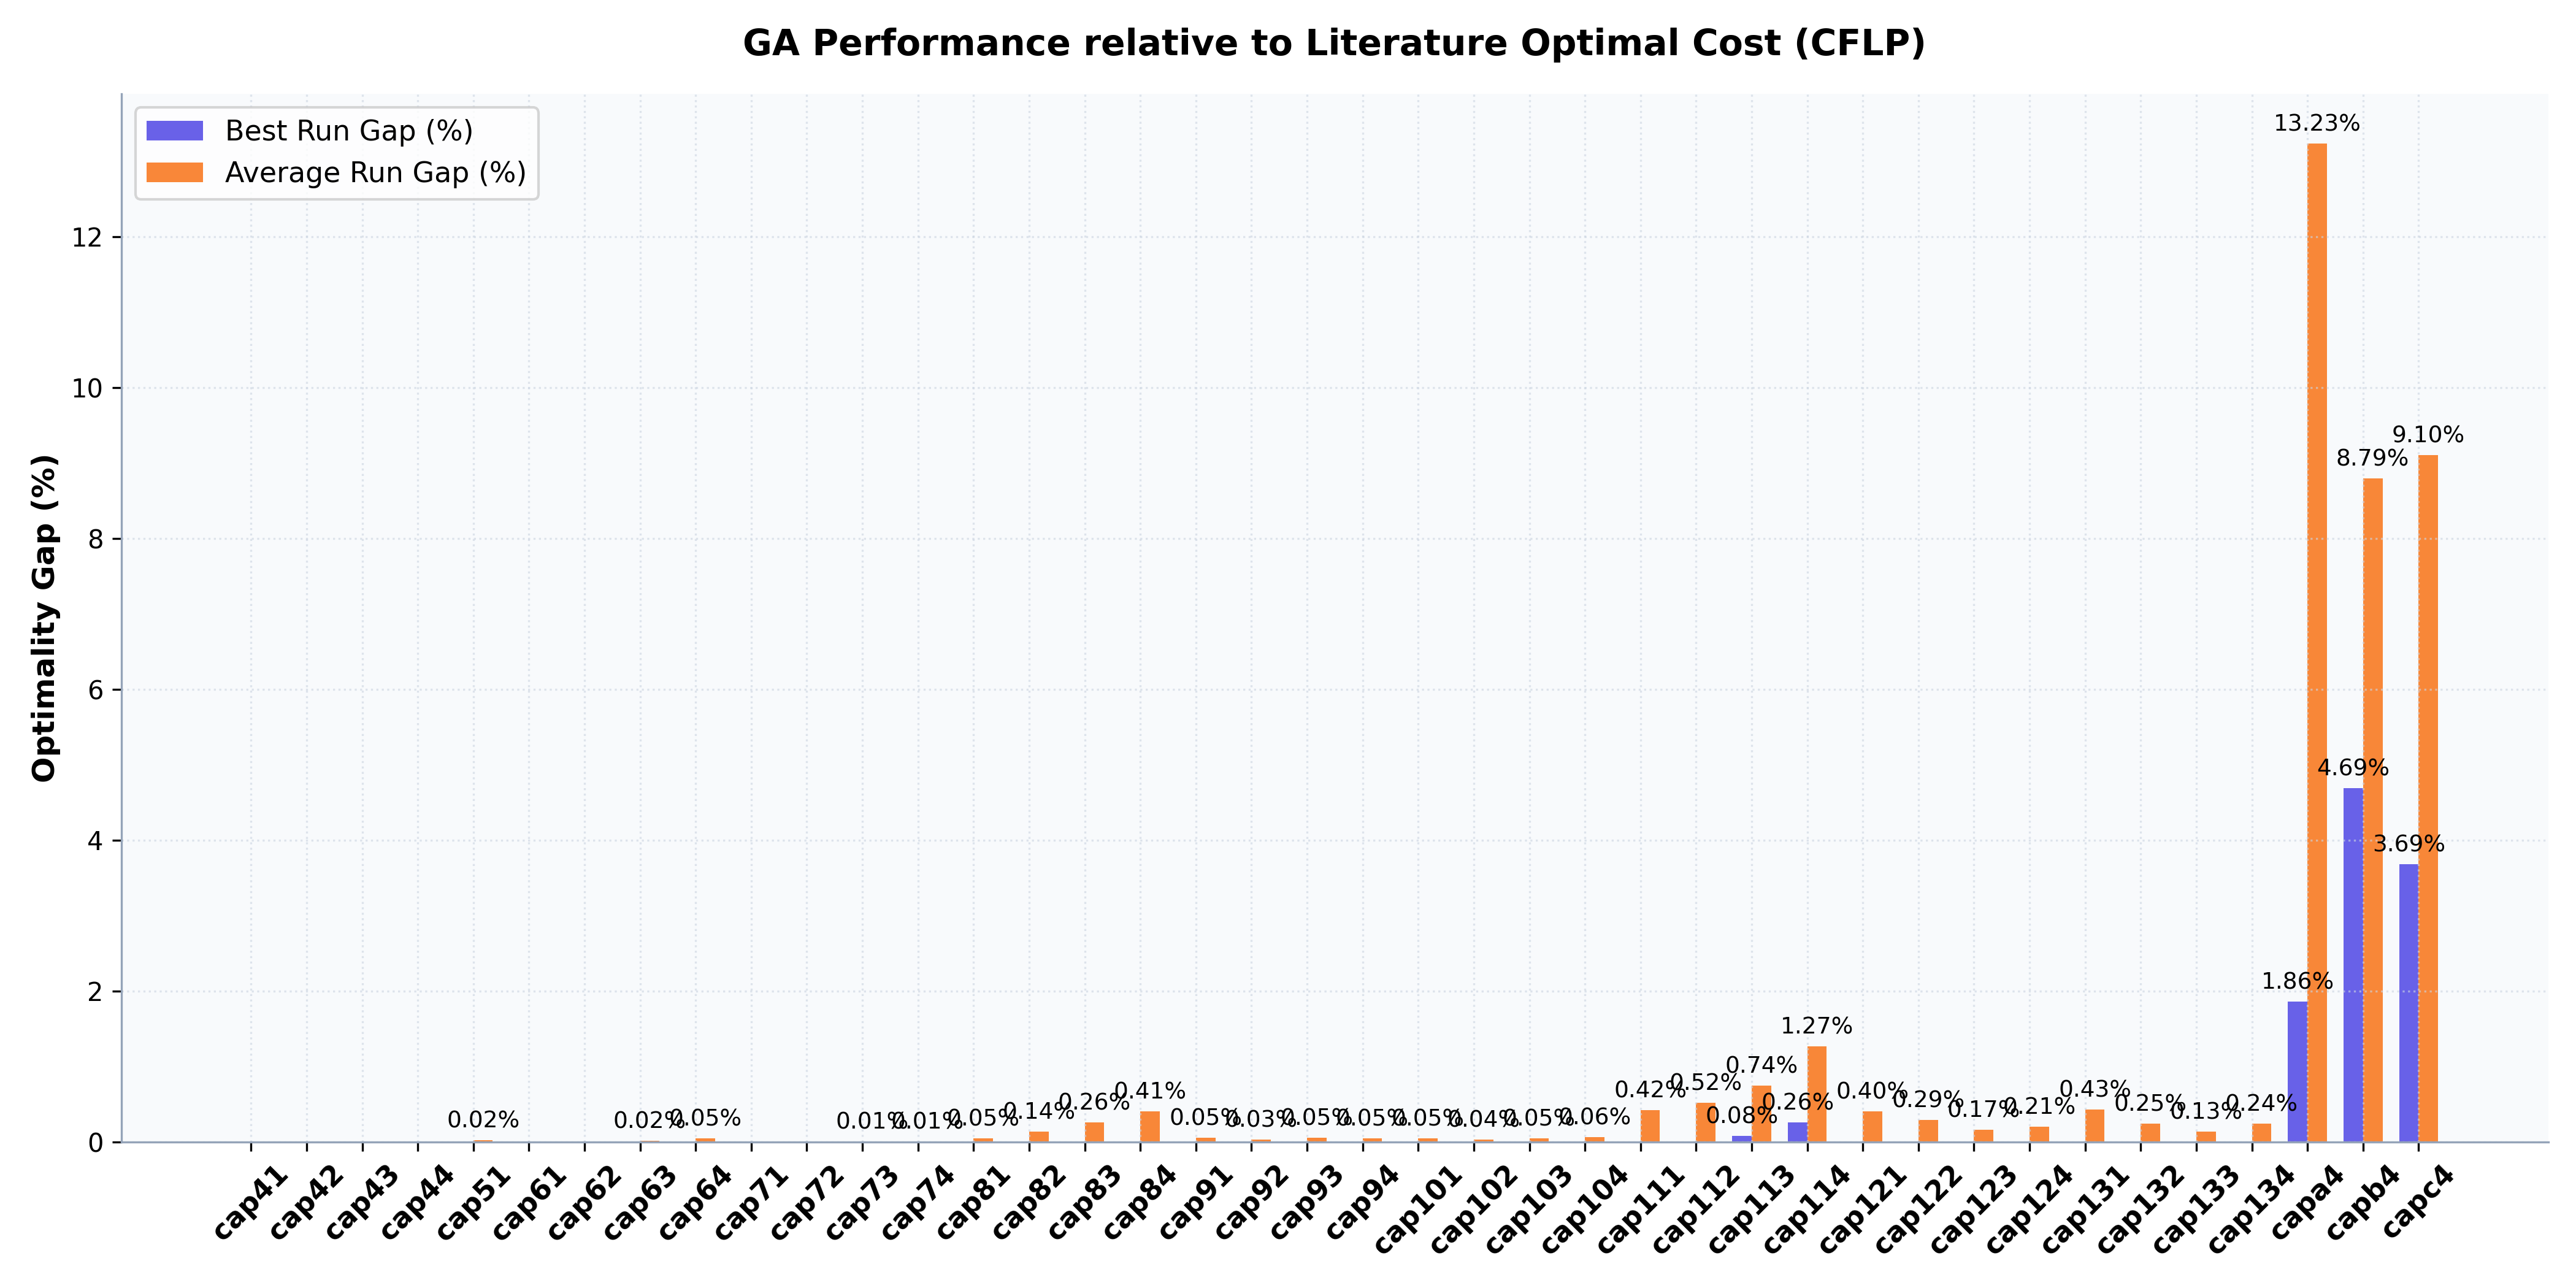
\includegraphics[width=\columnwidth]{statistical_benchmark_results.png}
\caption{Classical GA best-run and average-run optimality gap (\%) versus the published literature optimum, across all 40 OR-Library instances. Gaps are near zero throughout cap41--cap134 and grow sharply only on the three 100-facility instances (capa4/capb4/capc4).}
\label{fig:stat_bar}
\end{figure}

\subsection{Computational Cost Breakdown}

The optimality-gap tables above do not by themselves show \emph{why} the
Hybrid ML-GA is worth using when it is competitive: the surrogate changes how
many fitness evaluations are exact versus predicted, and this has a direct
runtime cost. Table~\ref{tab:runtime} reports, for the same representative
instances as Table~\ref{tab:full_classical}, the classical GA's total wall
time (across its full run budget -- 30 runs for small/medium instances, 10 for
the three large ones) against the Hybrid ML-GA's bootstrap time, surrogate
training time, and total solve-phase time (10 confidence-aware runs), plus the
average number of exact-LP versus surrogate evaluations actually performed
per solve run.

\begin{table}[t]
\centering
\caption{Computational cost breakdown (representative instances). Classical GA time is the full run budget (30 runs small/medium, 10 runs large); Hybrid ML-GA time is bootstrap + train + 10 solve runs. Evals columns are per-solve-run averages.}
\label{tab:runtime}
\resizebox{\columnwidth}{!}{
\begin{tabular}{lrrrrrr}
\toprule
\multirow{2}{*}{Instance} & Classical GA & \multicolumn{3}{c}{Hybrid ML-GA Time (s)} & \multicolumn{2}{c}{Avg.\ Evals / Run} \\
\cmidrule(lr){3-5} \cmidrule(lr){6-7}
 & Total Time (s) & Bootstrap & Train & Solve (10 runs) & Exact & Surrogate \\
\midrule
cap41  & 84.4    & 4.8   & 0.70 & 252.2 & 1{,}800.0 & 10{,}200.0 \\
cap83  & 401.7   & 6.0   & 0.68 & 313.3 & 1{,}800.0 & 10{,}200.0 \\
cap111 & 1{,}109.9 & 8.7  & 0.70 & 407.2 & 1{,}800.0 & 10{,}200.0 \\
cap134 & 8.5     & 0.14  & 0.89 & 98.6  & 1{,}800.0 & 10{,}200.0 \\
capa4  & 52.9    & 10.0  & 0.97 & 143.7 & 1{,}505.4 & 8{,}494.6 \\
capb4  & 165.3   & 9.1   & 1.07 & 201.4 & 1{,}523.3 & 8{,}476.7 \\
capc4  & 231.2   & 107.8 & 0.95 & 237.7 & 1{,}560.2 & 8{,}439.8 \\
\bottomrule
\end{tabular}}
\end{table}

Two patterns are visible that the optimality-gap tables alone do not surface.
First, across every small/medium instance, roughly 85\% of fitness
evaluations per solve run are handled by the surrogate rather than the exact
LP solver ($10{,}200$ of $12{,}000$ total evaluations at population 120 /
generation 100, after accounting for the warm-up period), confirming that the
confidence-aware policy is genuinely deferring most of the computational
burden to the surrogate rather than defaulting to exact evaluation. Second,
the classical GA's own total time varies by more than two orders of magnitude
across instances of similar facility count purely due to early-convergence
termination (\emph{cap134} stops after very few generations at $8.5$s total,
while \emph{cap111} runs much closer to its full generation budget at
$1{,}109.9$s) -- a further illustration that summary statistics computed from
a single run count can be misleading without the underlying per-instance
numbers reported alongside them. \emph{capc4}'s bootstrap time ($107.8$s) is
an outlier relative to \emph{capa4}/\emph{capb4} ($\sim$$10$s); this is
consistent with \emph{capc4}'s larger observed run-to-run variance elsewhere
in this study (Table~\ref{tab:xlarge}) and is noted here rather than smoothed
over.

\subsection{Convergence Behaviour}

Fig.~2 and Fig.~3 show representative convergence curves for \emph{cap41}
(16 facilities) for the classical GA and Hybrid ML-GA respectively. The
classical GA's best-cost curve drops to the published optimum by generation
$\sim$10 and holds there, while the population-average curve continues to
oscillate around a higher cost due to ongoing mutation and crossover
exploration. The Hybrid ML-GA's best-cost curve descends over a similar
number of generations to the same exact-verified final cost
(\$1{,}040{,}444.38), confirming that the confidence-aware policy converges
to the correct optimum on this instance despite most generations being
evaluated by the surrogate rather than the exact solver.

\begin{figure}[t]
\centering
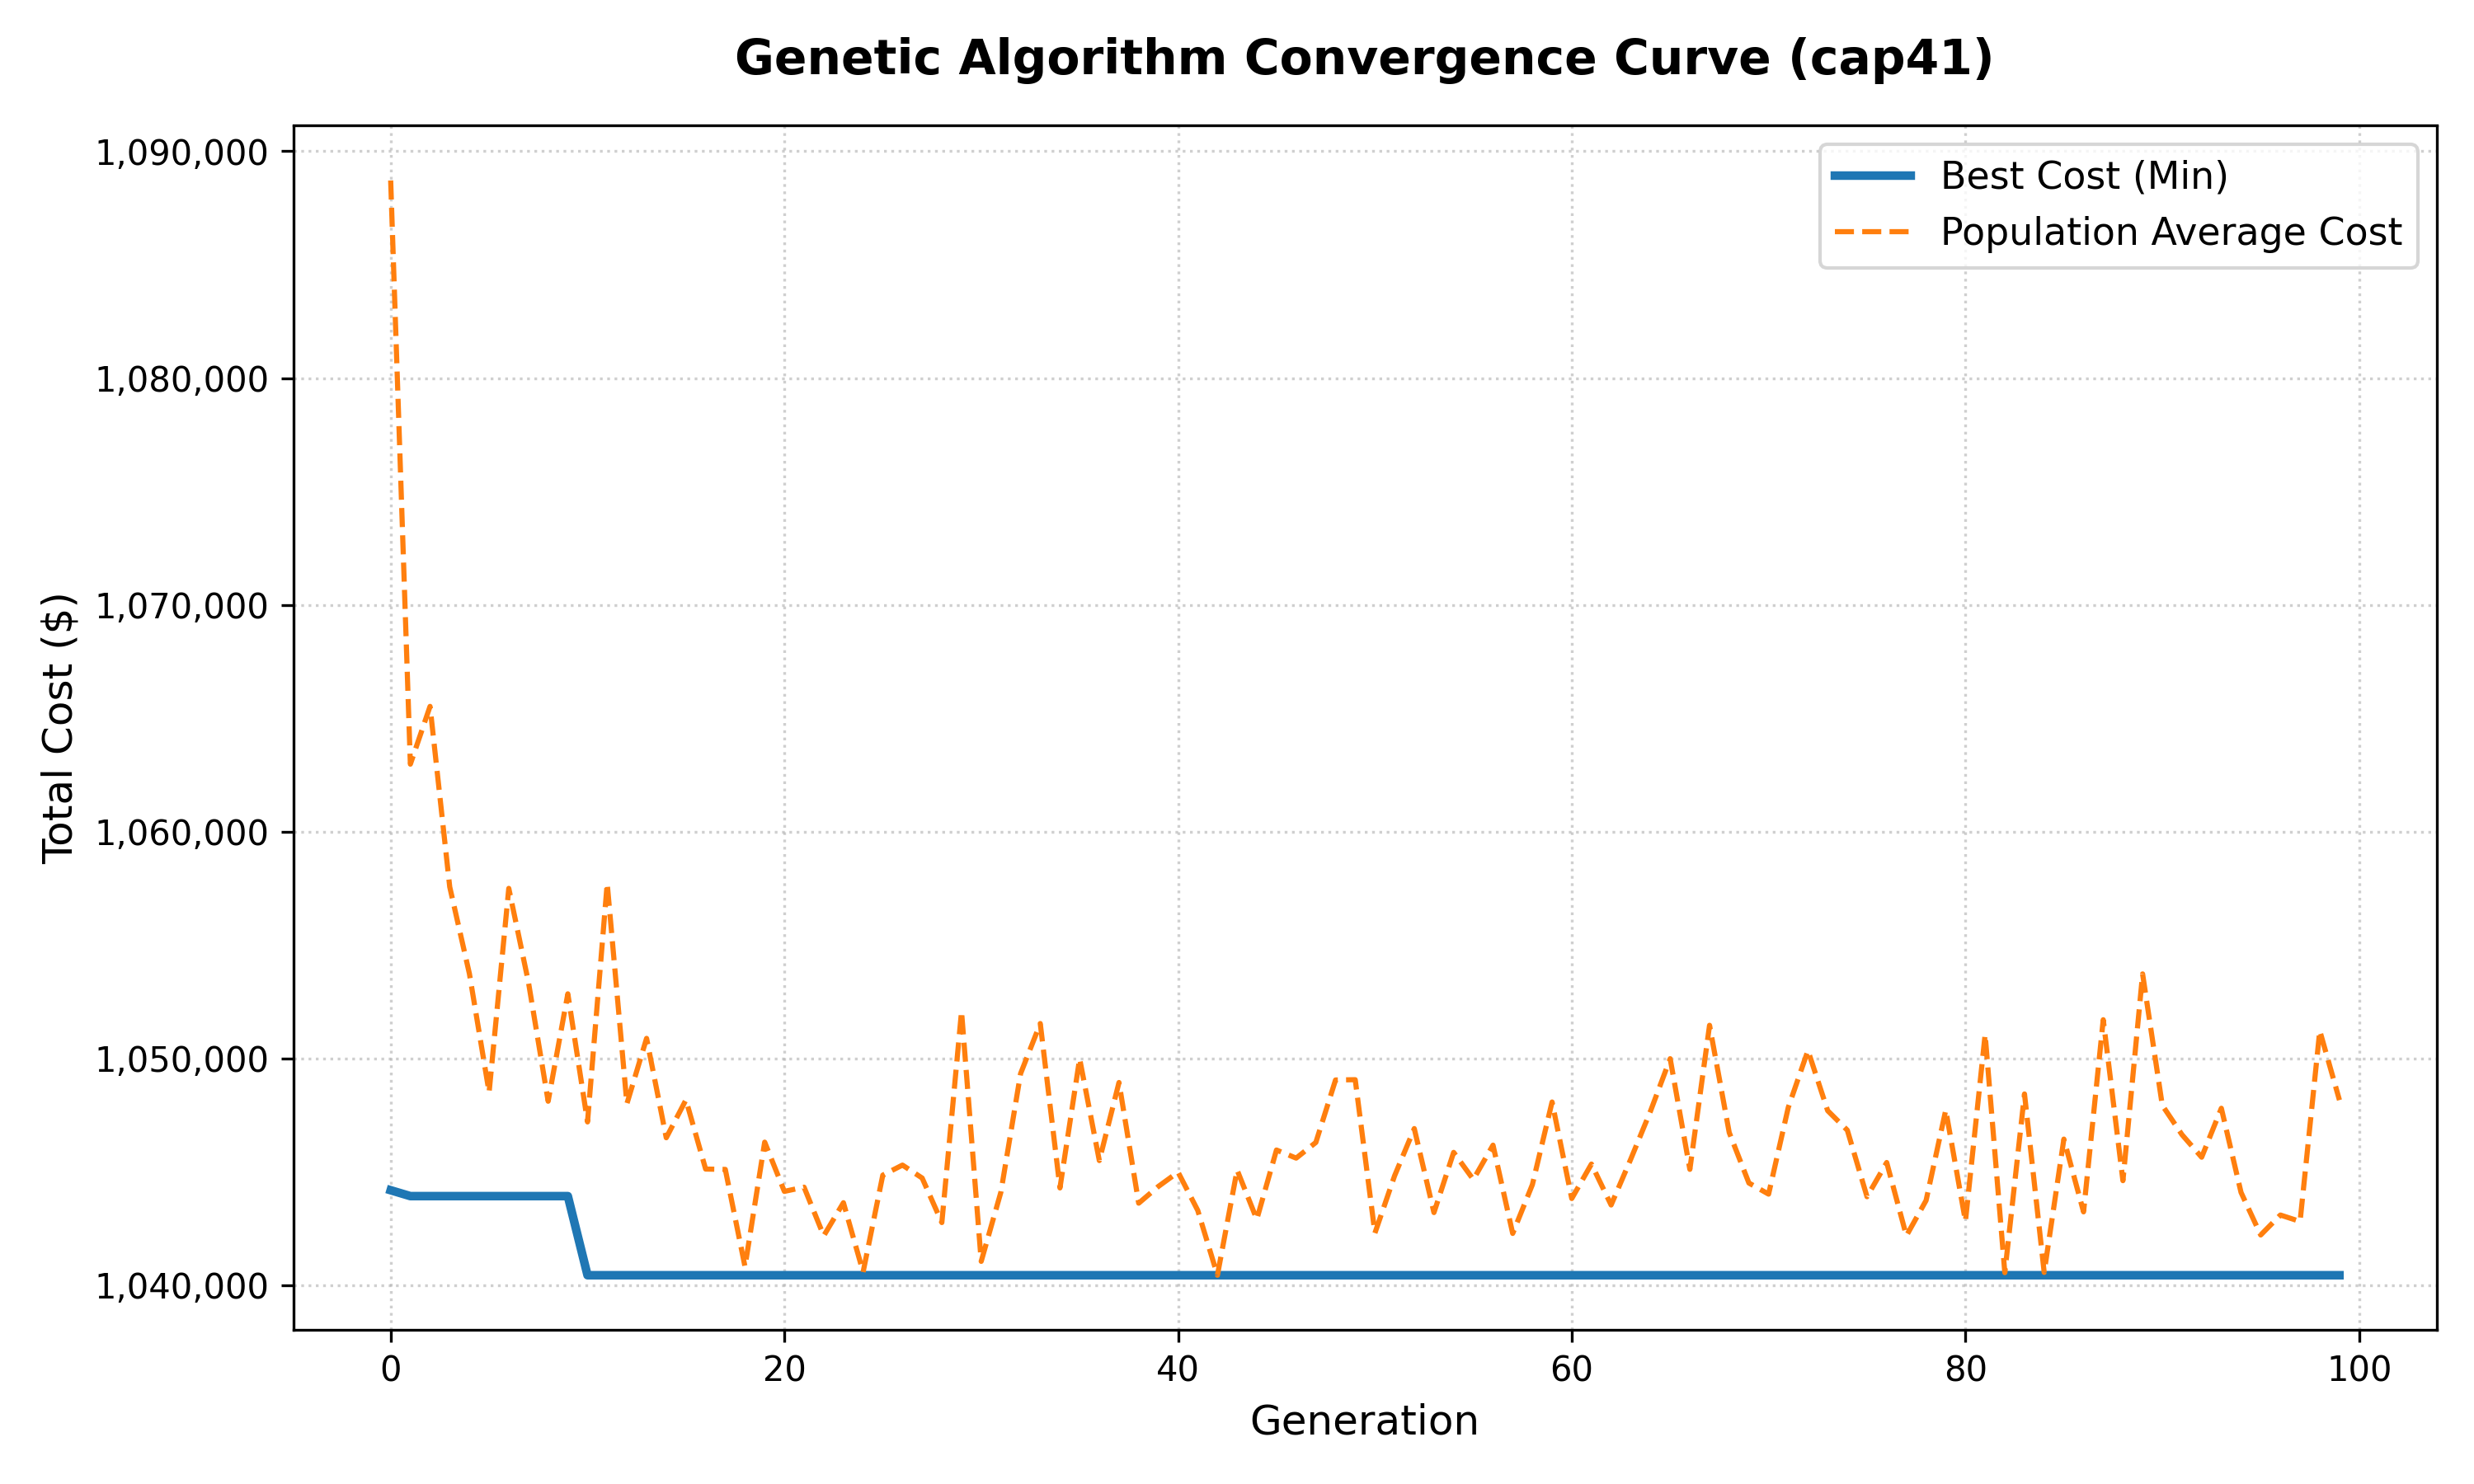
\includegraphics[width=\columnwidth]{cap41_ga_convergence.png}
\caption{Classical GA convergence on cap41: best cost (solid) and population-average cost (dashed) versus generation.}
\label{fig:ga_conv}
\end{figure}

\begin{figure}[t]
\centering
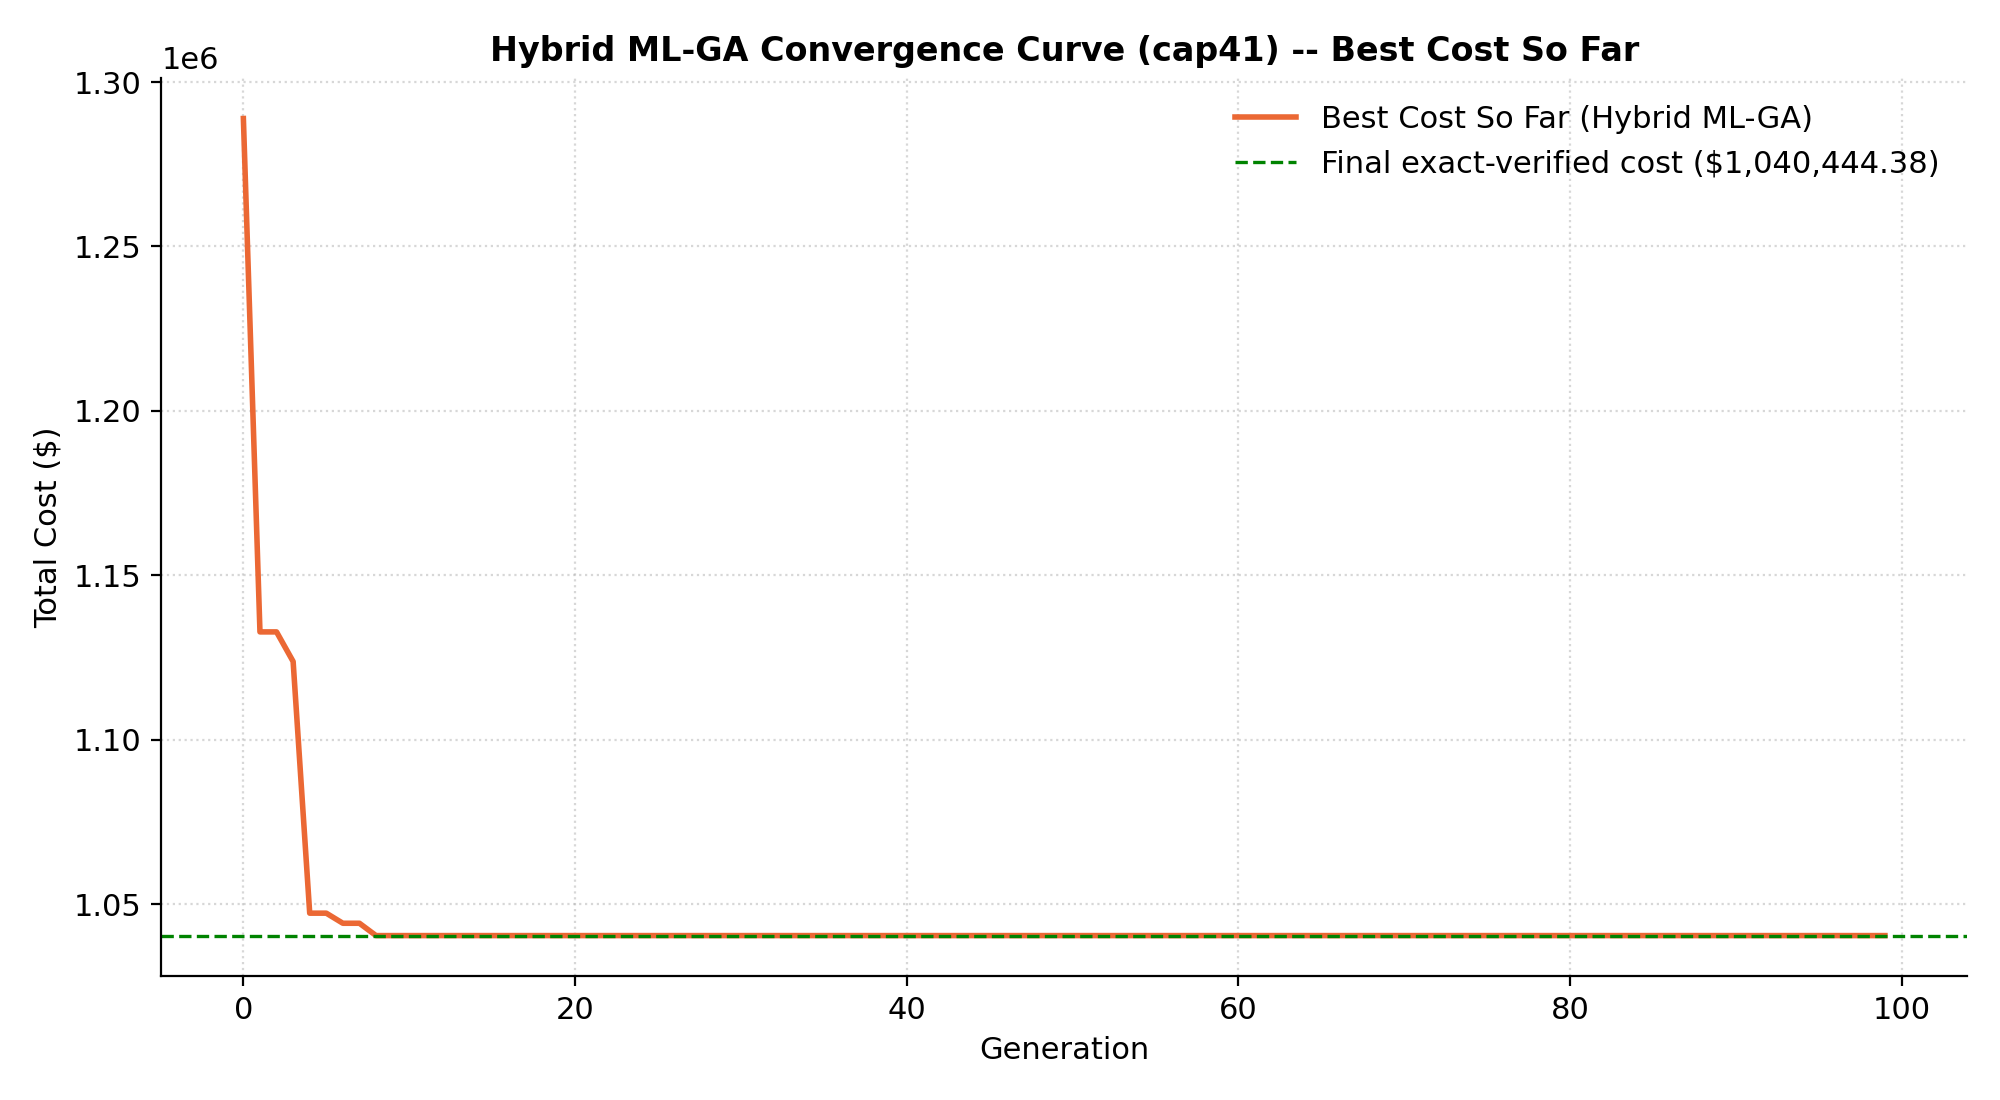
\includegraphics[width=\columnwidth]{cap41_hybrid_convergence.png}
\caption{Hybrid ML-GA convergence on cap41: best cost so far under the confidence-aware policy, converging to the same exact-verified cost as the classical GA.}
\label{fig:hybrid_conv}
\end{figure}

\emph{cap41} is only one of 40 instances, and a single case is not sufficient
to characterise convergence behaviour across the whole benchmark suite. To
check this, one representative run of each solver was executed on
\emph{every} OR-Library instance (the same pop/gen budgets as
Section~IV-A) and each run's best-cost-so-far trajectory was normalised by
its own final value, so that instances of very different absolute cost scale
can be compared on one shared axis. Fig.~4 and Fig.~5 show the resulting
small-multiple grids for the classical GA and Hybrid ML-GA respectively.

\begin{figure}[t]
\centering
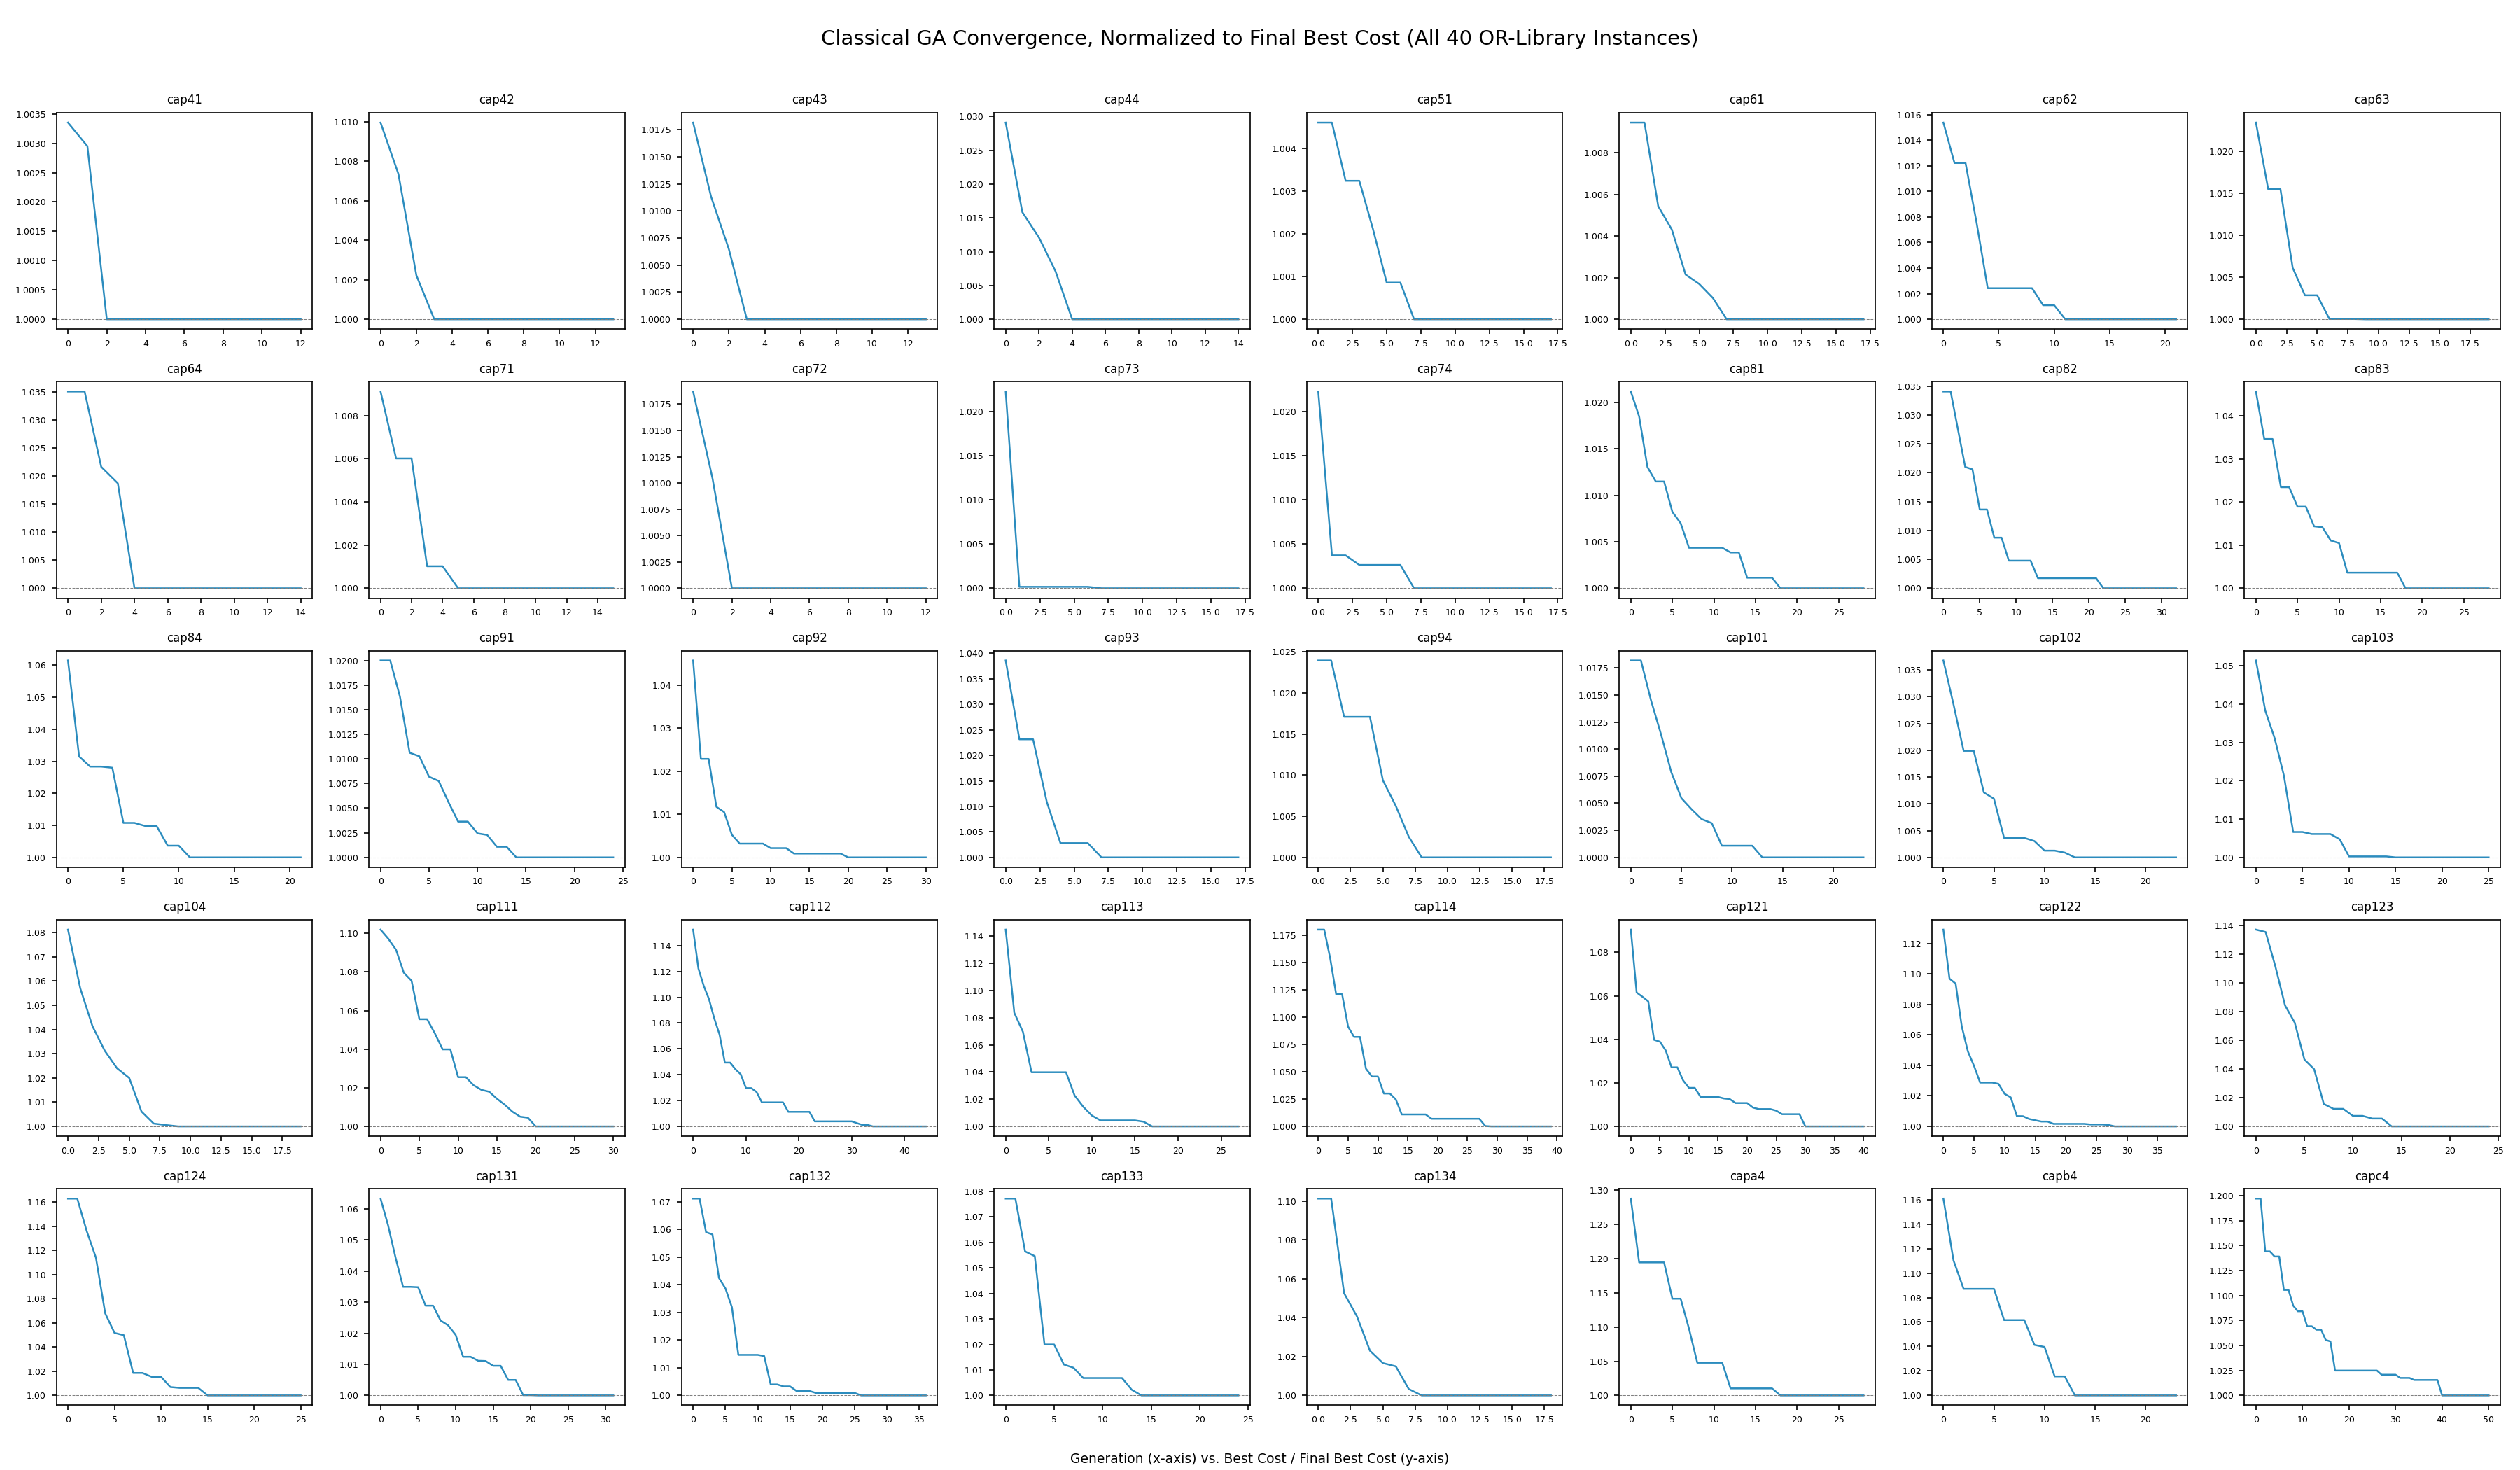
\includegraphics[width=\columnwidth]{all_instances_classical_convergence_grid.png}
\caption{Classical GA convergence on all 40 OR-Library instances (one representative run per instance, seed 42). Each panel plots best-cost-so-far normalised by that instance's own final value versus generation. Convergence to the normalised floor of $1.0$ takes visibly more generations as facility count grows from the top-left (\emph{cap41}, 16 facilities) toward the bottom-right (\emph{capa4}/\emph{capb4}/\emph{capc4}, 100 facilities).}
\label{fig:grid_classical}
\end{figure}

\begin{figure}[t]
\centering
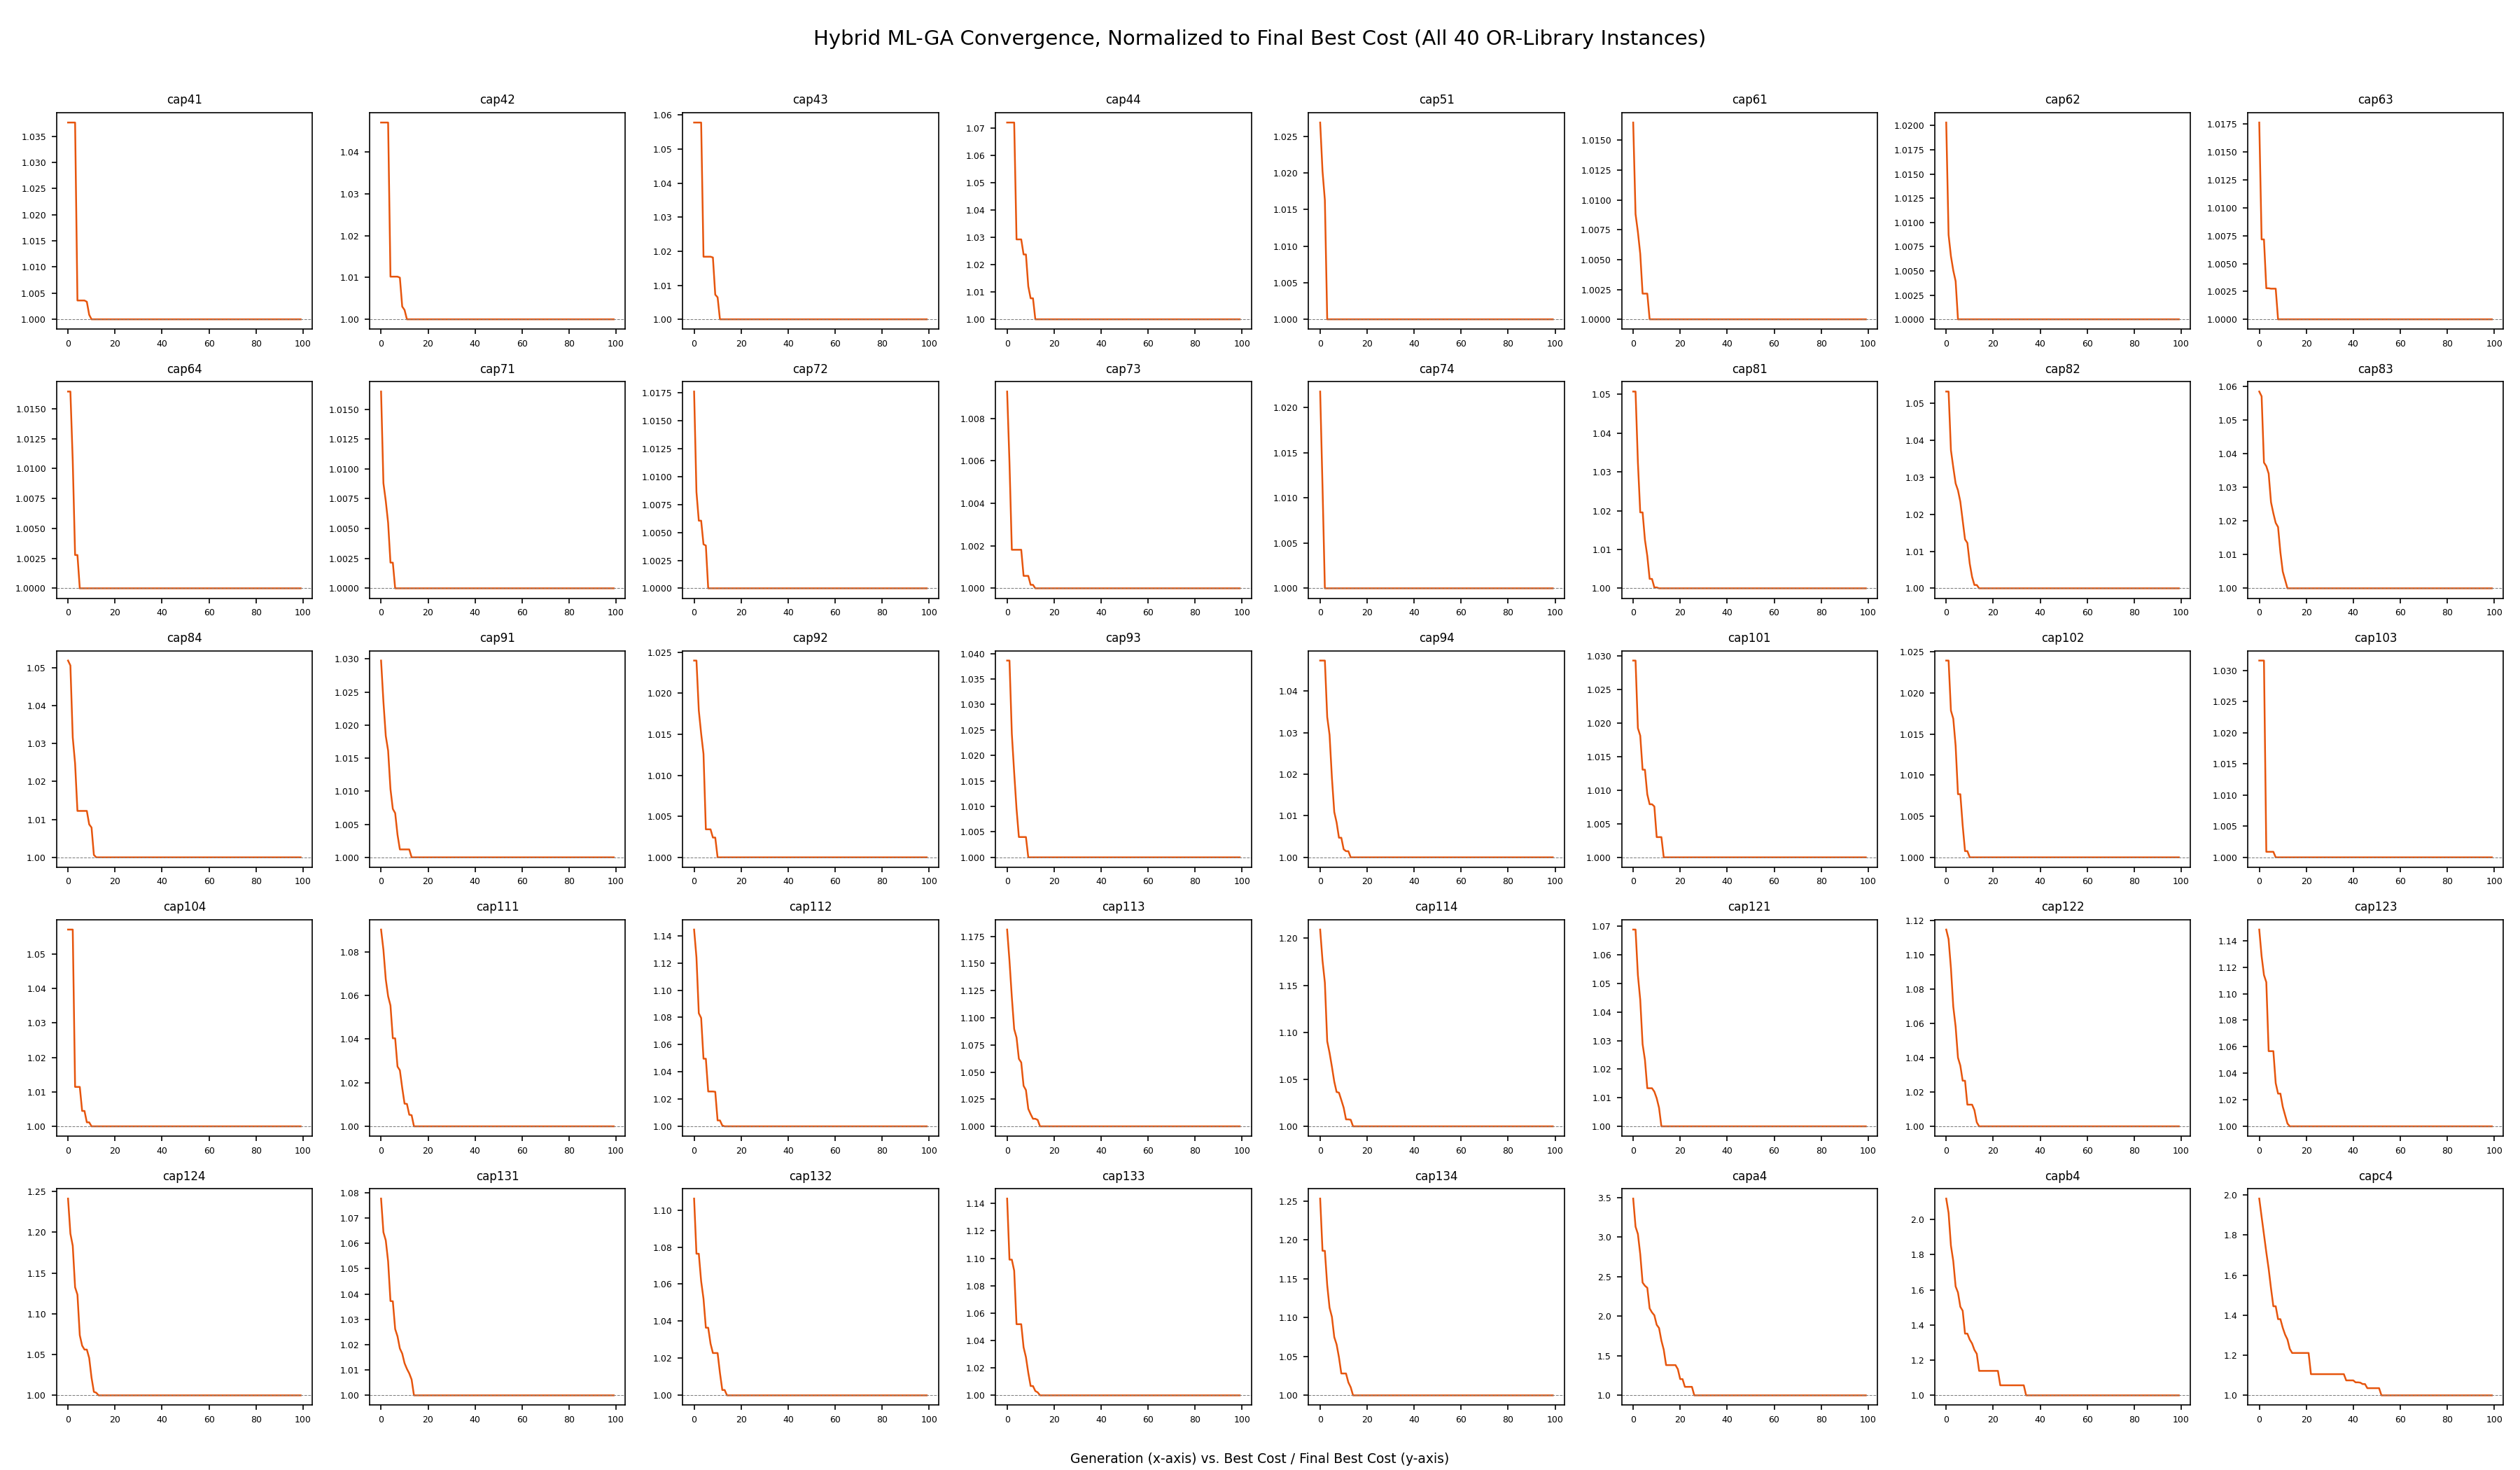
\includegraphics[width=\columnwidth]{all_instances_hybrid_convergence_grid.png}
\caption{Hybrid ML-GA convergence on all 40 OR-Library instances (one representative run per instance, seed 42), same normalisation as Fig.~4. Note the much taller initial-to-final ratio on \emph{capa4} ($3.5\times$), \emph{capb4} ($2.1\times$), and \emph{capc4} ($2.0\times$) compared to any small/medium instance ($\le 1.06\times$): the search has a proportionally much larger gap to close on the 100-facility instances. This quantifies how much harder those instances are for the surrogate-guided search; Section~V-B examines, and ultimately does not support, the natural explanation that the cause is simply an under-sized training corpus.}
\label{fig:grid_hybrid}
\end{figure}

Two patterns emerge that a single-instance plot cannot show. First, every
instance in both solvers converges monotonically to its normalised floor of
$1.0$ well within its generation budget, confirming that neither solver is
running out of generations before converging on any of the 40 instances --
the large-instance optimality gap reported in Table~\ref{tab:xlarge} is a
gap to a \emph{better solution the search did not reach}, not a sign that a
converging search was cut off early. Second, the \emph{initial} normalised
ratio (how far the first generation's best cost is from the final one) grows
sharply with instance size for the Hybrid ML-GA specifically: $\le 1.06\times$
for every 16--25-facility instance, up to $\sim$$1.2\times$ for the
50-facility group, and $2.0$--$3.5\times$ for the three 100-facility
instances -- a much steeper relative climb than the classical GA shows on the
same instances (Fig.~4). On the largest instances the surrogate's initial
guidance therefore starts proportionally further from the eventual answer,
leaving the confidence-aware policy more relative distance to close. It is
tempting to read this as direct evidence for the sampling-budget hypothesis of
Section~V-A -- the training corpus was not scaled up proportionally to
instance size -- but the experiment in Section~V-B shows that enlarging the
corpus does not in fact close the gap, so this figure should be read as
characterising \emph{how much} harder the large instances are for the
surrogate-guided search, not as establishing \emph{why}.

\subsection{Classical GA versus Hybrid ML-GA: All 40 Instances}

Fig.~6 compares best-run and average-run optimality gaps for both solvers
across all 40 instances. Table~\ref{tab:small}--\ref{tab:xlarge} report the
same comparison numerically, grouped by instance size, so that exact values
are available alongside the visual comparison.

\begin{figure}[t]
\centering
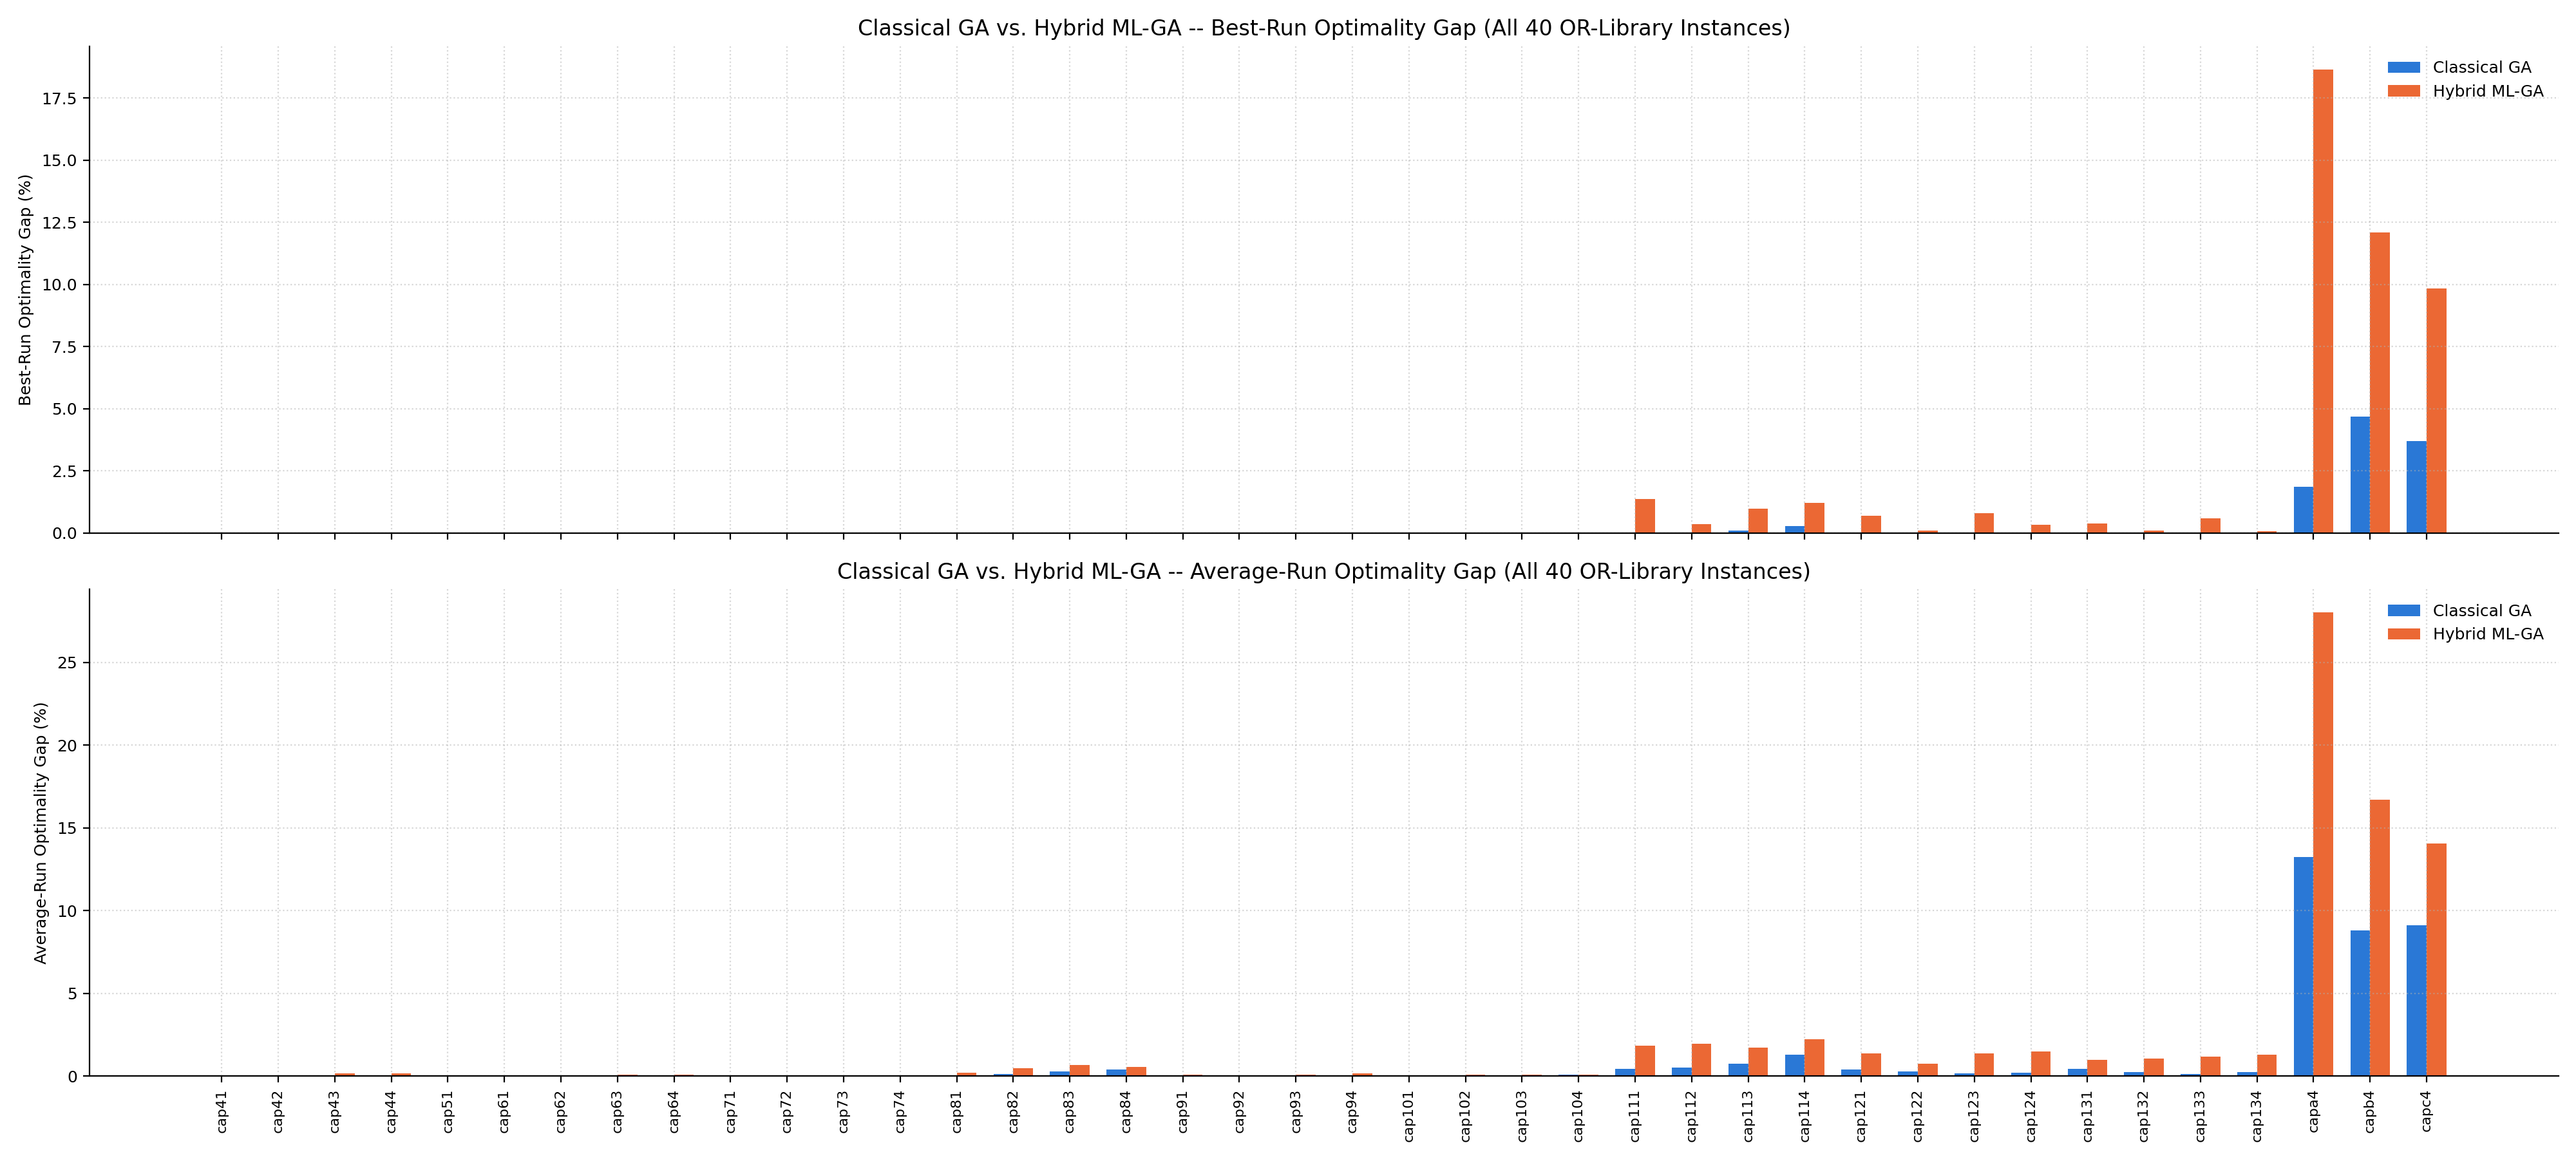
\includegraphics[width=\columnwidth]{fig6_classical_vs_hybrid_all_instances.png}
\caption{Classical GA vs.\ Hybrid ML-GA: best-run (top) and average-run (bottom) optimality gap (\%) across all 40 OR-Library instances. The two solvers are visually indistinguishable through cap41--cap104; the gap between them opens gradually across cap111--cap134 and becomes large on capa4/capb4/capc4.}
\label{fig:fig6}
\end{figure}

\begin{table}[t]
\centering
\caption{Optimality gaps (\%): small/medium instances (16--25 facilities).}
\label{tab:small}
\resizebox{\columnwidth}{!}{
\begin{tabular}{lcccc}
\toprule
Instance & Classical Best & Hybrid Best & Classical Avg & Hybrid Avg \\
\midrule
cap41 & 0.0000 & 0.0000 & 0.0000 & 0.0174 \\
cap42 & 0.0000 & 0.0000 & 0.0000 & 0.0000 \\
cap43 & 0.0000 & 0.0000 & 0.0000 & 0.1519 \\
cap44 & 0.0000 & 0.0000 & 0.0000 & 0.1418 \\
cap51 & 0.0000 & 0.0000 & 0.0214 & 0.0000 \\
cap61 & 0.0000 & 0.0000 & 0.0000 & 0.0170 \\
cap62 & 0.0000 & 0.0000 & 0.0000 & 0.0000 \\
cap63 & 0.0000 & 0.0000 & 0.0158 & 0.0798 \\
cap64 & 0.0000 & 0.0000 & 0.0482 & 0.0723 \\
cap71 & 0.0000 & 0.0000 & 0.0000 & 0.0170 \\
cap72 & 0.0000 & 0.0000 & 0.0000 & 0.0000 \\
cap73 & 0.0000 & 0.0000 & 0.0061 & 0.0363 \\
cap74 & 0.0000 & 0.0000 & 0.0088 & 0.0265 \\
cap81 & 0.0000 & 0.0000 & 0.0519 & 0.1985 \\
cap82 & 0.0000 & 0.0000 & 0.1353 & 0.4677 \\
cap83 & 0.0000 & 0.0000 & 0.2606 & 0.6748 \\
cap84 & 0.0000 & 0.0000 & 0.4051 & 0.5483 \\
cap91 & 0.0000 & 0.0000 & 0.0533 & 0.0680 \\
cap92 & 0.0000 & 0.0000 & 0.0350 & 0.0558 \\
cap93 & 0.0000 & 0.0000 & 0.0544 & 0.0881 \\
cap94 & 0.0000 & 0.0000 & 0.0515 & 0.1502 \\
cap101 & 0.0000 & 0.0000 & 0.0520 & 0.0570 \\
cap102 & 0.0000 & 0.0000 & 0.0358 & 0.0941 \\
cap103 & 0.0000 & 0.0000 & 0.0473 & 0.0638 \\
cap104 & 0.0000 & 0.0000 & 0.0608 & 0.0938 \\
\bottomrule
\end{tabular}}
\end{table}

\begin{table}[t]
\centering
\caption{Optimality gaps (\%): large-scaled instances (50 facilities).}
\label{tab:large50}
\resizebox{\columnwidth}{!}{
\begin{tabular}{lcccc}
\toprule
Instance & Classical Best & Hybrid Best & Classical Avg & Hybrid Avg \\
\midrule
cap111 & 0.0000 & 1.3585 & 0.4242 & 1.8439 \\
cap112 & 0.0000 & 0.3562 & 0.5209 & 1.9669 \\
cap113 & 0.0834 & 0.9798 & 0.7436 & 1.7202 \\
cap114 & 0.2613 & 1.2106 & 1.2693 & 2.2163 \\
cap121 & 0.0000 & 0.6893 & 0.4038 & 1.3668 \\
cap122 & 0.0000 & 0.0895 & 0.2923 & 0.7598 \\
cap123 & 0.0000 & 0.7791 & 0.1654 & 1.3792 \\
cap124 & 0.0000 & 0.3204 & 0.2062 & 1.4963 \\
cap131 & 0.0000 & 0.3767 & 0.4286 & 0.9613 \\
cap132 & 0.0000 & 0.0896 & 0.2474 & 1.0623 \\
cap133 & 0.0000 & 0.5767 & 0.1346 & 1.1550 \\
cap134 & 0.0000 & 0.0559 & 0.2418 & 1.2712 \\
\bottomrule
\end{tabular}}
\end{table}

\begin{table}[t]
\centering
\caption{Optimality gaps (\%): extremely large-scaled instances (100 facilities, 1000 customers).}
\label{tab:xlarge}
\begin{tabular}{lcccc}
\toprule
Instance & Classical Best & Hybrid Best & Classical Avg & Hybrid Avg \\
\midrule
capa4 & 1.8634 & 18.6533 & 13.2337 & 28.0084 \\
capb4 & 4.6877 & 12.0801 & 8.7925 & 16.7110 \\
capc4 & 3.6858 & 9.8240 & 9.0996 & 14.0591 \\
\bottomrule
\end{tabular}
\end{table}

Both solvers find the published optimum in their best run on every
small/medium instance (Table~\ref{tab:small}); the difference between them
appears only in the average-run column, where the surrogate introduces
additional run-to-run variance (up to $0.67\%$ versus the classical GA's
$0.41\%$). On the 50-facility group (Table~\ref{tab:large50}) the classical GA
reaches the optimum in its best run on 10 of 12 instances and stays within
$0.26\%$ on the rest, while the Hybrid ML-GA's best-run gaps range
$0.06$--$1.36\%$. On the 100-facility group (Table~\ref{tab:xlarge}) the
classical GA clearly outperforms the Hybrid ML-GA; this is the central
negative finding of the study and is analysed in Section~V-A.

\subsection{Surrogate Fit Quality}

Fig.~7 reports the Random Forest surrogate's held-out $R^2$ for all 40
instances, clipped to $[-1, 1]$ for readability (\emph{cap83}'s true value is
$-3.6\times10^{10}$ and would otherwise compress every other bar to
invisibility). 34 of 40 instances achieve $R^2 \ge 0.68$, reaching $0.99$ on
the three large instances. Of the remaining six, four (\emph{cap61},
\emph{cap62}, \emph{cap63}, and \emph{cap83}) show degenerate or strongly
negative $R^2$, traced to a small number of heavily capacity-penalised
chromosomes surviving into an already-small bootstrap-derived training corpus
for those specific instances; the other two (\emph{cap94} at $0.39$ and
\emph{cap103} at $0.68$) are simply weak rather than degenerate fits.

\begin{figure}[t]
\centering
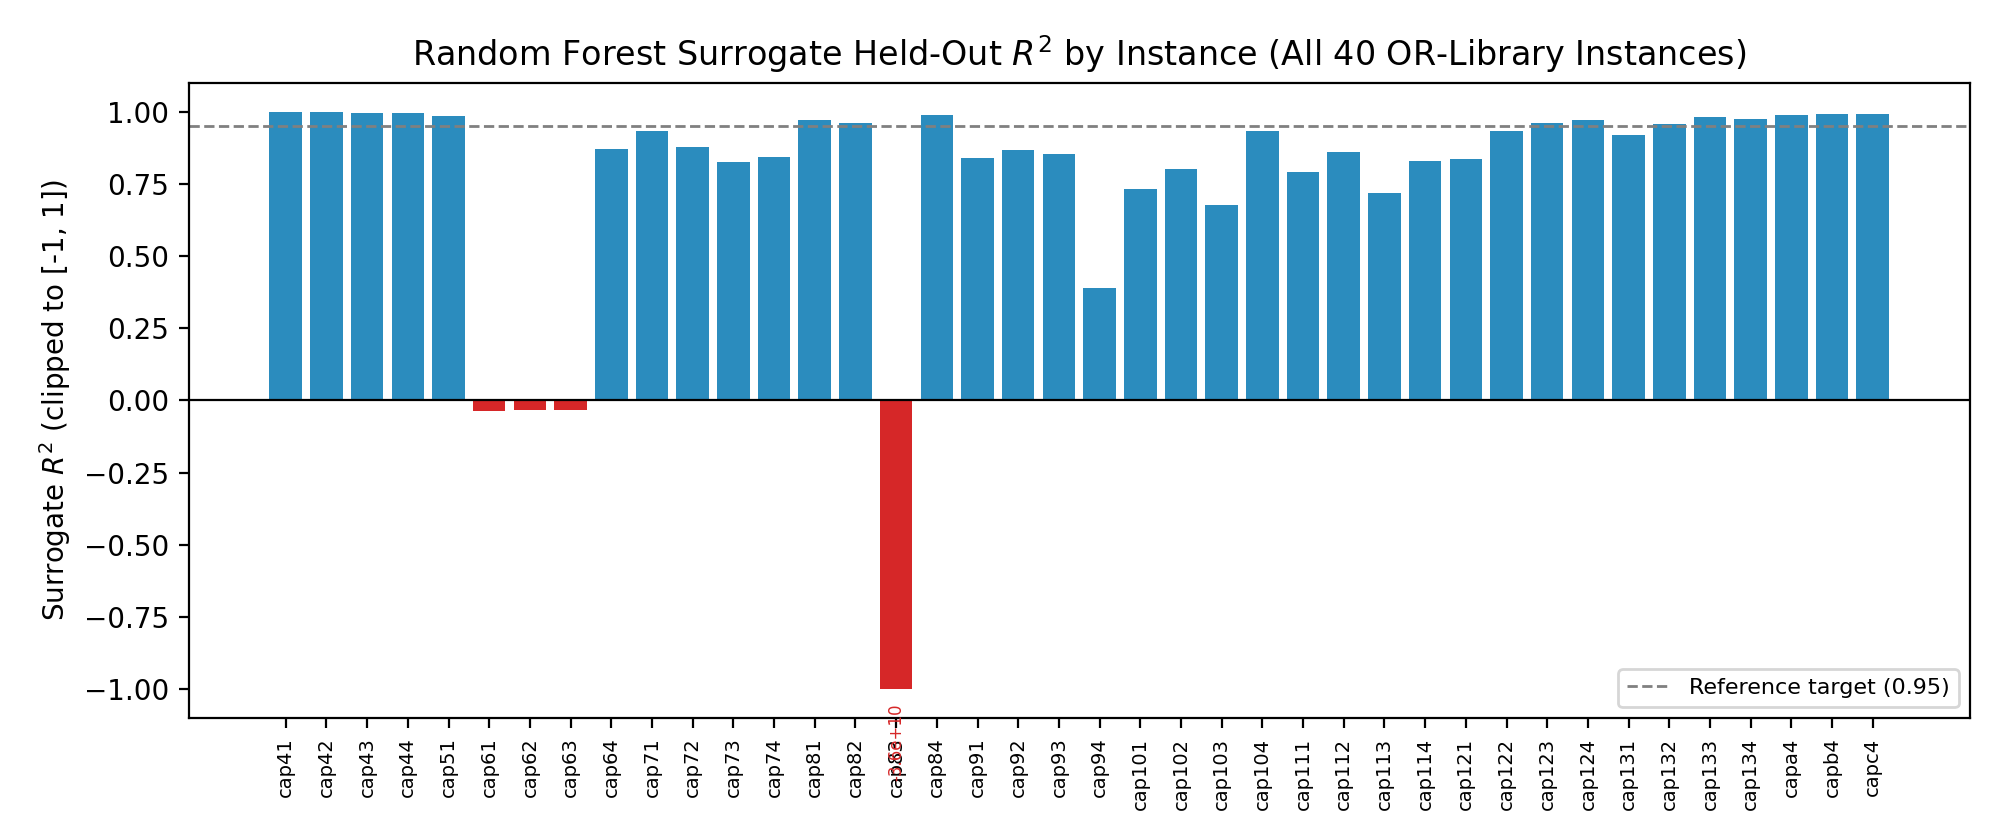
\includegraphics[width=\columnwidth]{fig_surrogate_r2_clipped.png}
\caption{Random Forest surrogate held-out $R^2$ per instance, clipped to $[-1,1]$. Bars in red fall below zero; \emph{cap83}'s unclipped value is annotated. Despite four instances with poor surrogate fit, none of them show a degraded final best-run gap (Section V-A), because the confidence-aware policy verifies exactly whenever the surrogate would otherwise matter. Note that a high $R^2$ here does \emph{not} imply accurate cost prediction: Section~IV-G shows that on ten of these instances $R^2$ exceeds $0.99$ while MAPE exceeds $100\%$.}
\label{fig:r2}
\end{figure}

\subsection{Surrogate Architecture Comparison and the Limits of $R^2$}

The results above use a Random Forest surrogate throughout. To test whether
that choice is justified, all four implemented architectures (Random Forest,
Gradient Boosting, XGBoost, and a multilayer perceptron) were trained and
evaluated on the identical cached bootstrap corpus of every one of the 40
instances, so the comparison isolates the architecture and holds the training
data fixed. Table~\ref{tab:surrogate_arch} reports the aggregate results.

\begin{table}[t]
\centering
\caption{Surrogate architecture comparison across all 40 instances, trained on identical per-instance bootstrap corpora. ``Fails'' counts instances whose MAPE exceeds $100\%$. Speed-up is relative to an exact LP evaluation.}
\label{tab:surrogate_arch}
\resizebox{\columnwidth}{!}{
\begin{tabular}{lrrrrr}
\toprule
Architecture & Med.\ MAPE & Max MAPE & Fails & Med.\ $R^2$ & Med.\ speed-up \\
\midrule
Random Forest & 1.41\% & 948{,}600\% & 10/40 & 0.899 & 5.2$\times$ \\
Gradient Boosting & 1.20\% & \textbf{5.5\%} & \textbf{0/40} & 0.927 & 320$\times$ \\
XGBoost & \textbf{1.14\%} & 11{,}974\% & 2/40 & \textbf{0.936} & 262$\times$ \\
MLP & 14.81\% & 99.5\% & 0/40 & $-3.000$ & 823$\times$ \\
\bottomrule
\end{tabular}}
\end{table}

Three findings follow, the first of which qualifies how the $R^2$ values in
Fig.~\ref{fig:r2} should be read.

\textbf{$R^2$ is a misleading accuracy metric for this surrogate task.} On the
ten instances where the bootstrap corpus contains Big-M capacity penalties,
the Random Forest attains an apparently excellent $R^2$ (e.g.\ $0.998$ on
\emph{cap41}) while its MAPE on the same predictions is $521{,}100\%$. The two
metrics disagree because the penalty values are several orders of magnitude
larger than genuine solution costs, so they dominate the total sum of squares
that $R^2$ normalises against: a model can capture almost all of that
penalty-driven variance, and thereby score a near-perfect $R^2$, while being
wrong by a factor of thousands on the ordinary-cost chromosomes that actually
matter to the search. Fig.~\ref{fig:r2} should therefore be read as a
diagnostic of variance capture, not of predictive accuracy on the cost scale;
the MAPE column of Table~\ref{tab:surrogate_arch} is the more meaningful
measure.

\textbf{Gradient Boosting is the only architecture that never fails.} Its
worst MAPE across all 40 instances is $5.5\%$, whereas Random Forest exceeds
$100\%$ MAPE on 10 instances and XGBoost on 2. The MLP is unusable, with
negative $R^2$ on 37 of 40 instances.

\textbf{Random Forest is also the slowest at inference by a wide margin.} Its
median speed-up over an exact LP evaluation is $5.2\times$, against
$320\times$ for Gradient Boosting and $262\times$ for XGBoost -- roughly a
$60\times$ difference. Since accelerating fitness evaluation is the entire
motivation for introducing a surrogate, this is a substantial penalty.

Taken together, the architecture used for every headline result in this paper
is the weakest of the three tree-based options on both accuracy and speed.
The natural inference is that the reported results understate the framework's
capability and that re-running the benchmark under Gradient Boosting would
improve them. Section~IV-H tests that inference directly.

\subsection{Does a Better Surrogate Produce Better Solutions?}

Section~IV-G establishes that Gradient Boosting is a far more accurate
surrogate than the Random Forest used for the headline results -- a bounded
worst-case MAPE of $5.5\%$ against $948{,}600\%$. If surrogate accuracy drives
solution quality, substituting it should measurably improve the reported gaps.
This was tested under a strictly controlled swap: identical cached bootstrap
corpora, identical seed sequence (42--51), identical population and generation
budgets, with the surrogate architecture as the only difference.
Table~\ref{tab:rf_vs_gb} reports the outcome.

\begin{table}[t]
\centering
\caption{Hybrid ML-GA under a Random Forest versus a Gradient Boosting surrogate, all else held identical. Despite a five-order-of-magnitude difference in worst-case surrogate MAPE, no group shows a significant difference in solution quality.}
\label{tab:rf_vs_gb}
\resizebox{\columnwidth}{!}{
\begin{tabular}{lrrrr}
\toprule
Instance group & Classical & RF & GB & Wilcoxon RF vs.\ GB \\
 & mean gap & mean gap & mean gap & $p$-value \\
\midrule
Small/medium (16--25 fac.) & 0.055\% & 0.1248\% & 0.1204\% & 0.066 \\
Large (50 fac.) & 0.390\% & 1.4333\% & 1.4333\% & 1.000 \\
Extremely large (100 fac.) & 10.375\% & 19.593\% & 19.026\% & 0.393 \\
\midrule
Overall (all 40) & 0.929\% & 1.9774\% & 1.9322\% & 0.326 \\
\bottomrule
\end{tabular}}
\end{table}

The improvement is negligible and statistically insignificant everywhere:
$p = 0.326$ overall, and no group reaches significance at $\alpha = 0.05$. The
prediction implied by Section~IV-G is not borne out.

Inspecting the raw per-seed costs explains why, and is more informative than
the aggregate. \textbf{On 33 of the 40 instances the two architectures produce
\emph{bit-identical} final costs on all ten seeds.} Replacing a surrogate whose
predictions are wrong by a factor of thousands with one accurate to within
$5.5\%$ changed the returned solution on no seed of no instance in that
majority; only 7 instances (\emph{cap61}, \emph{cap63}, \emph{cap64},
\emph{cap71}, and the three 100-facility instances) differ at all.

This identifies a structural property of the confidence-aware policy that the
aggregate gap tables cannot show. Under that policy the incumbent best is
updated only after an exact LP verification, so the returned solution is always
one the exact evaluator has confirmed; the surrogate's only influence is over
\emph{which} candidates are put forward for verification. A prediction that is
too high causes a good candidate to be passed over silently, and a prediction
that is too low is caught by the verification gate before it can affect the
result. The surrogate can therefore lose good solutions but never contribute
one, and its accuracy is largely decoupled from the quality of what the search
ultimately returns.

This is consistent with established findings in the surrogate-assisted
evolutionary algorithm literature, and is best understood as confirming and
sharpening them rather than as a new discovery. Two prior results are directly
pertinent. Theoretically, Chen et al.\ \citep{chen2013} analyse a
surrogate-assisted evolutionary algorithm in which candidates are pre-evaluated
by a surrogate and precisely evaluated with probability $p$ when the
pre-evaluation ranks them worse than the incumbent. They show that the
acceleration obtained decreases monotonically with $p$, and that surrogate
pre-evaluation can prevent convergence to the global optimum by screening out
good candidates. The confidence-aware policy studied here is precisely the
$p = 0$ case of that scheme: a candidate predicted no better than the incumbent
is never verified. Chen et al.'s analysis therefore predicts both halves of what
is observed -- maximal computational saving, and a mechanism by which good
solutions can be silently lost -- and the present results supply an empirical
confirmation of that prediction on a real constrained combinatorial problem.
Empirically, Hanawa et al.\ \citep{hanawa2025} report that individual-based and
generation-based model management ``exhibit robust performance when the accuracy
surpasses a certain threshold,'' i.e.\ that improving an already-adequate
surrogate ceases to improve the search. The present result extends that in a
specific and practically relevant way. Their finding is a threshold effect established on
continuous benchmarks with a pseudo-surrogate of tunable accuracy, and it
predicts degradation once accuracy falls \emph{below} the threshold. Here the
decoupling holds even for a surrogate that is catastrophically inaccurate --
\emph{cap41}'s Random Forest has a MAPE of $521{,}100\%$, and \emph{cap41} is
nonetheless among the 33 bit-identical instances. Mandatory exact verification
before any incumbent update therefore confers a robustness that does not depend
on the surrogate clearing an accuracy threshold at all, which a threshold
account alone does not predict.

That decoupling also accounts for both negative results in this study under a
single mechanism. Section~V-B finds that improving the surrogate through active
learning does not improve solution quality; this section finds that replacing
the surrogate with a far more accurate architecture does not either. Neither is
an isolated anomaly: both follow from a decision rule that, by construction,
insulates the reported solution from the surrogate almost entirely. The
policy's conservatism is what makes the framework safe -- a badly fit surrogate
cannot corrupt a reported result, as \emph{cap83} demonstrates -- and it is
also what caps the framework's achievable solution quality at that of the
underlying exact-LP GA. The value the surrogate delivers is therefore
\emph{computational}, in displacing exact LP calls, and not qualitative. A
framework seeking genuine solution-quality gains from a surrogate would need a
decision rule that allows well-calibrated predictions to influence selection
directly, accepting some risk in exchange for the possibility of gain.

\subsection{Comparison Against an Exact MILP Baseline}

To contextualise the 100-facility results against an exact reference beyond
the published literature optimum, the classical GA, a greedy heuristic, and an
MILP solver (CBC, 180-second time limit) were compared on the 12
disaggregated 100-facility variants. Table~\ref{tab:milp} reports the
results.

\begin{table}[t]
\centering
\caption{MILP, Greedy, and Classical GA on the 100-facility variants. MILP gap is vs.\ published ground truth; Greedy/GA gaps are vs.\ the time-limited MILP cost (negative = beat MILP within its time limit).}
\label{tab:milp}
\resizebox{\columnwidth}{!}{
\begin{tabular}{lccc}
\toprule
Instance & MILP Gap vs.\ GT (\%) & Greedy Gap vs.\ MILP (\%) & GA Gap vs.\ MILP (\%) \\
\midrule
capa1 & 1.36 & 28.52 & 12.06 \\
capa2 & 5.70 & 35.48 & 9.04 \\
capa3 & 11.29 & 32.40 & $-$5.23 \\
capa4 & 19.94 & 28.32 & $-$11.47 \\
capb1 & 5.78 & 25.45 & 3.56 \\
capb2 & 14.43 & 1.83 & $-$6.55 \\
capb3 & 15.60 & 0.58 & $-$8.30 \\
capb4 & 12.17 & 7.01 & $-$7.05 \\
capc1 & 12.53 & 19.22 & 0.06 \\
capc2 & 10.53 & 20.91 & $-$0.57 \\
capc3 & 11.27 & 18.70 & $-$1.08 \\
capc4 & 12.36 & 8.03 & $-$4.53 \\
\bottomrule
\end{tabular}}
\end{table}

CBC cannot close the branch-and-bound gap within its time limit on any of the
12 instances and is reported honestly as ``feasible, not proven optimal''
rather than falsely labelled optimal. MILP remains the closest of the three
methods to the published ground truth on all 12 instances; the classical GA
finds a cheaper solution than the time-limited MILP solver on 8 of 12
instances -- a legitimate outcome since MILP's reported cost here is a
feasible upper bound, not a proven optimum.

\subsection{Statistical Significance Testing}

The comparisons above report descriptive statistics. To establish whether the
observed differences between the two solvers are statistically meaningful
rather than sampling noise, both solvers were re-run under a \emph{matched}
protocol: 10 independent runs per instance per solver using the identical seed
sequence (42--51), on all 40 instances, giving 400 paired observations. This
matched design is what makes a paired test valid, and it removes the unequal
run-count obstacle (30 versus 10) that prevented such a test in an earlier
version of this study. Following the methodology of the base study
\citep{ozsoydan2023} and the recommendations of Derrac et al.\
\citep{derrac2011}, the non-parametric Wilcoxon signed-rank test is applied,
pairing each seed's classical-GA optimality gap against the Hybrid ML-GA gap
on the same instance and seed. Table~\ref{tab:wilcoxon} reports the results.

\begin{table}[t]
\centering
\caption{Wilcoxon signed-rank test on paired per-seed optimality gaps (10 matched seeds per instance, classical GA vs.\ Hybrid ML-GA).}
\label{tab:wilcoxon}
\resizebox{\columnwidth}{!}{
\begin{tabular}{lrrrrl}
\toprule
Instance group & Pairs & Classical & Hybrid & $p$-value & Result at $\alpha=0.05$ \\
 & & mean gap & mean gap & & \\
\midrule
Small/medium (16--25 fac.) & 250 & 0.055\% & 0.125\% & $1.4\times10^{-2}$ & Significant \\
Large (50 fac.) & 120 & 0.390\% & 1.433\% & $3.3\times10^{-19}$ & Significant \\
Extremely large (100 fac.) & 30 & 10.375\% & 19.593\% & $2.0\times10^{-7}$ & Significant \\
\midrule
Overall (all 40) & 400 & 0.929\% & 1.977\% & $1.2\times10^{-25}$ & Significant \\
\bottomrule
\end{tabular}}
\end{table}

The null hypothesis of equal medians is rejected in every instance group and
overall, with the classical GA achieving the lower mean gap in all four cases.
This is a more precise -- and less favourable -- statement than the
descriptive comparison in Section~IV-E supports on its own, and it warrants a
careful reading on the small/medium group in particular. There, the difference
is statistically significant ($p = 0.014$) but practically negligible: mean
gaps of $0.055\%$ versus $0.125\%$ mean both solvers land within roughly one
eighth of one percent of the published optimum, and both recover the exact
optimum in their best run on every instance in that group
(Table~\ref{tab:small}). Statistical significance here reflects the
consistency of a very small difference across 250 paired observations, not a
difference of practical consequence. On the 50- and 100-facility groups, by
contrast, the difference is both statistically significant and practically
large -- a $3.7\times$ and $1.9\times$ higher mean gap respectively -- and it
is these groups that motivate the analysis in Section~V.

\section{Discussion}

\subsection{Root Cause of the Large-Instance Gap}

The Hybrid ML-GA's underperformance on the three largest instances was
investigated directly. An initial probe using a small bootstrap budget
(population 30, 15 generations, 450 exact evaluations) produced a 148\%
optimality gap on a 100-facility instance -- far too sparse a sample relative
to the combinatorial size of a 100-dimensional binary search space to train a
useful surrogate. Increasing the bootstrap budget to population 60 / 40
generations (2{,}400 exact evaluations) and the solve-phase budget to
population 100 / 100 generations reduced the gap to the range reported in
Table~\ref{tab:xlarge}, but not to parity with the classical GA. The
surrogate's held-out $R^2$ on these three instances is high ($0.99$),
indicating a good fit \emph{in-distribution}.

This observation suggests a natural hypothesis: that the limiting factor is
sampling budget rather than model quality -- that 1{,}500--2{,}400 GA-derived
training samples characterise only a small neighbourhood of a 100-facility
search space, insufficient to guide 100 generations of evolutionary search
toward a near-optimal region outside that neighbourhood. If that were the
whole story, enlarging the corpus and improving the surrogate's fit should
narrow the gap. Section~V-B reports a direct experimental test of exactly that
prediction, and the result does not support it.

On the four instances with degenerate surrogate $R^2$ (\emph{cap61},
\emph{cap62}, \emph{cap63}, \emph{cap83}), this poor fit did not propagate
into a worse final result: \emph{cap83}'s own best-run gap is $0\%$. This
follows directly from the confidence-aware decision rule: a surrogate
prediction is only trusted unverified when it does not claim a new best
solution, so a poorly fit surrogate that occasionally predicts nonsensical
costs is filtered out by the exact-verification gate whenever it matters,
rather than allowed to corrupt the reported result.

\subsection{Testing the Sampling-Budget Hypothesis via Active Learning}

The quality-gated active-learning loop of Section~III-F provides a direct test
of the hypothesis stated in Section~V-A. Applied to the three 100-facility
instances for five rounds each, it repeatedly runs the Hybrid ML-GA, feeds the
resulting exact evaluations back into the training corpus, retrains, and
adopts the retrained surrogate only if its $R^2$ on a fixed held-out
validation set does not regress. The final adopted surrogate was then
evaluated under the identical protocol used for the headline results (10
confidence-aware runs, seeds 42--51, population 100 / 100 generations), so
pre- and post-active-learning numbers are directly comparable.
Table~\ref{tab:active_learning} reports the outcome.

\begin{table}[t]
\centering
\caption{Active learning on the three 100-facility instances: five rounds each. The corpus grows roughly tenfold and surrogate $R^2$ improves on all three instances, yet the resulting optimality gap improves on only one.}
\label{tab:active_learning}
\resizebox{\columnwidth}{!}{
\begin{tabular}{lrrrrrr}
\toprule
\multirow{2}{*}{Instance} & \multicolumn{2}{c}{Corpus size} & \multicolumn{2}{c}{Surrogate $R^2$} & \multicolumn{2}{c}{Best gap (\%)} \\
\cmidrule(lr){2-3} \cmidrule(lr){4-5} \cmidrule(lr){6-7}
 & before & after & before & after & before & after \\
\midrule
capa4 & 718 & 7{,}342 & 0.9901 & 0.9976 & 18.65 & 25.59 \\
capb4 & 736 & 7{,}056 & 0.9920 & 0.9972 & 12.08 & \textbf{8.44} \\
capc4 & 762 & 6{,}994 & 0.9926 & 0.9965 & 9.82 & 14.86 \\
\bottomrule
\end{tabular}}
\end{table}

The hypothesis predicts that all three gaps should narrow. Instead the gap
narrows on \emph{capb4} (12.08\% to 8.44\%) but widens on \emph{capa4}
(18.65\% to 25.59\%) and \emph{capc4} (9.82\% to 14.86\%) -- and it does so
even though the intervention worked exactly as designed on its own terms: the
corpus grew by roughly a factor of ten on every instance, and the surrogate's
validation $R^2$ improved on every instance. More training data and a
better-fitting surrogate did not produce better optimisation outcomes. The
sampling-budget explanation is therefore at best incomplete, and this study
reports that rather than retaining the more comfortable original
interpretation.

Two mechanisms plausibly account for the discrepancy, and distinguishing them
is left to future work. First, the quality gate is measured against a
validation set carved once from the \emph{initial} bootstrap corpus and
deliberately held fixed thereafter, so that $R^2$ remains comparable across
rounds. That design choice is correct for its stated purpose, but it means the
gate rewards fit to the initial sampling distribution, while the corpus itself
is progressively augmented with samples drawn from wherever the search has
since travelled. A model can thus score better and better on the gate while
becoming no better -- or worse -- in the regions where it is actually queried.
Second, and consistent with Section~IV-G, $R^2$ is itself a weak proxy for
predictive accuracy on the cost scale when the target distribution contains
extreme penalty values; a gate built on $R^2$ may therefore admit models whose
MAPE has deteriorated. Both mechanisms point to the same corrective direction:
the adoption criterion should be evaluated on a rolling validation set drawn
from the current search distribution, and should be based on MAPE rather than
$R^2$.

\subsection{Implementation Defects Found and Corrected During Verification}

Two defects were identified during verification and are reported here for
transparency, since all reported results reflect the corrected
implementation. \textbf{Template-file data corruption}: Beasley's OR-Library
distributes \emph{capa.txt}/\emph{capb.txt}/\emph{capc.txt} as unfilled
templates in which every facility's capacity field is the literal placeholder
text \texttt{"capacity"}. An earlier parser version silently substituted a
near-infinite placeholder capacity instead of raising an error, which would
have converted three of the benchmark's largest instances into an
artificially uncapacitated problem; the parser now raises an explicit error
naming the correctly instantiated replacement files (\emph{capa4},
\emph{capb4}, \emph{capc4}), used throughout this paper. \textbf{Thread-safety
native crash}: an earlier classical GA version parallelised fitness
evaluation across a thread pool for instances above 50 facilities, reliably
producing segmentation faults traced to SciPy's HiGHS backend not being safe
for concurrent multi-threaded invocation. Fitness evaluation is now
sequential for all instance sizes, which is slower -- the reason the
classical GA's large-instance configuration in Section~IV-A uses a reduced
budget relative to the small/medium configuration -- but eliminates the
crash.

\subsection{Limitations}

Several limitations qualify the results above. First, while Section~IV-H shows
that surrogate architecture has no significant effect on solution quality under
the current decision rule, that finding is established for two tree-based
architectures on this problem class and should not be generalised to decision
rules that permit unverified predictions to influence selection, where
surrogate accuracy would be expected to matter considerably more. Second, the
Wilcoxon tests of Section~IV-J use 10 matched runs per instance; while this is
sufficient to reject the null hypothesis decisively in every group, a larger
matched run count would tighten the effect-size estimates, and the Friedman
and Nemenyi post-hoc procedures used by the base study \citep{ozsoydan2023}
are not applied here because only two methods are being compared pairwise
rather than three or more. Third, the active-learning experiment
(Section~V-B) covers only the three 100-facility instances and a single
configuration (five rounds, $R^2$-gated adoption); the two candidate
explanations offered for its outcome are not experimentally separated, and the
corrective variants proposed there -- a rolling validation set and a
MAPE-based adoption criterion -- remain untested. Finally, all reported
results derive from a single hardware configuration and a fixed base random
seed, so absolute runtimes are indicative rather than portable.

\section{Conclusion and Future Directions}

This paper studied a surrogate-assisted extension of the binary/continuous
CFLP decomposition strategy established by Ozsoydan and G\"{o}lc\"{u}k
\citep{ozsoydan2023}: a machine learning surrogate trained directly from a
genetic algorithm's own search trajectory, via a bootstrap mechanism, is used
for the majority of fitness evaluations, with the exact solver reserved for
candidates whose predicted cost suggests a new best solution. Benchmarked
across all 40 Beasley OR-Library CFLP instances with full per-run statistics
rather than best-case summaries alone, the Hybrid ML-GA recovers the published
optimum in its best run on every instance up to 25 facilities, but Wilcoxon
signed-rank tests on 400 matched paired runs establish the classical exact-LP
GA as significantly better in every size group -- negligibly so on the small
and medium instances (mean gaps $0.055\%$ vs.\ $0.125\%$), substantially so on
the three 100-facility instances ($10.4\%$ vs.\ $19.6\%$).

The most useful contributions of this study are its negative results, which
converge on a single conclusion neither was designed to find. An
active-learning extension that enlarged the training corpus roughly tenfold and
improved surrogate $R^2$ on all three large instances nevertheless worsened the
optimality gap on two of them. Independently, substituting a surrogate five
orders of magnitude more accurate in worst-case MAPE changed nothing
statistically ($p = 0.33$) and produced bit-identical solutions on 33 of 40
instances. Two different routes to a better surrogate both failed to yield a
better solver.

The common cause is structural rather than incidental. Under the
confidence-aware policy the incumbent is updated only after exact LP
verification, so the surrogate governs only which candidates are put forward
for checking: it can pass over a good solution, but it can never contribute one
the exact evaluator has not already confirmed. Surrogate accuracy is therefore
largely decoupled from solution quality, and the framework's benefit is
computational -- displacing exact LP calls -- rather than qualitative. This is
a favourable property for trustworthiness, since a badly fit surrogate cannot
corrupt a reported result, but it caps achievable solution quality at that of
the underlying exact-LP GA and explains why the Hybrid ML-GA does not surpass
it in any instance group.

Three directions follow, reordered by what the evidence now supports. First,
and most substantively, revisit the decision rule itself: a policy that permits
well-calibrated predictions to influence selection directly -- accepting
bounded risk in exchange for the possibility of gain -- is the only route to
solution-quality improvement that these results leave open, and Gradient
Boosting's bounded $5.5\%$ worst-case MAPE suggests the calibration needed to
attempt it is attainable. Second, rebuild the active-learning adoption gate
around a rolling validation set drawn from the current search distribution and
scored by MAPE rather than $R^2$, addressing both mechanisms hypothesised in
Section~V-B. Third, since the surrogate's demonstrated benefit is speed,
evaluate the framework explicitly on a time-to-target basis rather than a
fixed-generation basis, which would measure the dimension on which it actually
delivers. A further direction, consistent with \citep{ozsoydan2023}'s own
future-work discussion, is coupling the framework with demand or cost
forecasting under uncertainty, extending toward stochastic and robust CFLP
variants \citep{saif2021,rahmati2021}.

\section*{Data Availability}

All benchmark instances are publicly available from Beasley's OR-Library
(\url{http://people.brunel.ac.uk/~mastjjb/jeb/orlib/capinfo.html}). Raw
per-run results accompany this paper: aggregate benchmarks in
\texttt{statistical\_benchmark\_results.csv},
\texttt{hybrid\_benchmark\_results.csv} and
\texttt{large\_benchmark\_results.csv}; the 400 matched paired runs underlying
the Wilcoxon tests in \texttt{raw\_runs\_all.csv} with test output in
\texttt{significance\_test\_results.json}; per-generation convergence
trajectories for all 40 instances in \texttt{all\_convergence\_data.csv}; the
four-way architecture comparison in \texttt{surrogate\_comparison.csv}; the
per-round active-learning history in
\texttt{active\_learning\_progress.json}; and the controlled Random Forest
versus Gradient Boosting comparison of Section~IV-H in
\texttt{rf\_vs\_gb\_comparison.csv}, with test output in
\texttt{rf\_vs\_gb\_tests.json}.

\bibliographystyle{IEEEtran}
\begin{thebibliography}{99}

\bibitem{ozsoydan2023} F. B. Ozsoydan and İ. Gölcük, ``A hybridisation of linear programming and genetic algorithm to solve the capacitated facility location problem,'' \emph{International Journal of Production Research}, vol. 61, no. 10, pp. 3331--3349, 2023.

\bibitem{beasley1988} J. E. Beasley, ``An algorithm for solving large capacitated warehouse location problems,'' \emph{European Journal of Operational Research}, vol. 33, no. 3, pp. 314--325, 1988.

\bibitem{christofides1983} N. Christofides and J. E. Beasley, ``Extensions to a Lagrangean relaxation approach for the capacitated warehouse location problem,'' \emph{European Journal of Operational Research}, vol. 12, no. 1, pp. 19--28, 1983.

\bibitem{contreras2010} I. Contreras, E. Fernández, and A. Marín, ``The tree of hubs location problem,'' \emph{European Journal of Operational Research}, vol. 202, no. 2, pp. 390--400, 2010.

\bibitem{vanroy1986} T. J. Van Roy, ``A cross decomposition algorithm for capacitated facility location,'' \emph{Operations Research}, vol. 34, no. 1, pp. 145--163, 1986.

\bibitem{wentges1996} P. Wentges, ``Accelerating Benders' decomposition for the capacitated facility location problem,'' \emph{Mathematical Methods of Operations Research}, vol. 44, no. 2, pp. 267--290, 1996.

\bibitem{klose2007} A. Klose and S. Görtz, ``A branch-and-price algorithm for the capacitated facility location problem,'' \emph{European Journal of Operational Research}, vol. 179, no. 3, pp. 1109--1125, 2007.

\bibitem{fischetti2016} M. Fischetti, I. Ljubić, and M. Sinnl, ``Benders decomposition without separability: A computational study for capacitated facility location problems,'' \emph{European Journal of Operational Research}, vol. 253, no. 3, pp. 557--569, 2016.

\bibitem{sun2012} M. Sun, ``A tabu search heuristic procedure for the capacitated facility location problem,'' \emph{Journal of Heuristics}, vol. 18, no. 1, pp. 91--118, 2012.

\bibitem{guastaroba2012} G. Guastaroba and M. G. Speranza, ``Kernel search for the capacitated facility location problem,'' \emph{Journal of Heuristics}, vol. 18, no. 6, pp. 877--917, 2012.

\bibitem{matos2021} T. Matos, Ó. Oliveira, and D. Gamboa, ``RAMP algorithms for the capacitated facility location problem,'' \emph{Annals of Mathematics and Artificial Intelligence}, vol. 89, no. 8, pp. 799--813, 2021.

\bibitem{rahmani2014} A. Rahmani and S. A. MirHassani, ``A hybrid firefly-genetic algorithm for the capacitated facility location problem,'' \emph{Information Sciences}, vol. 283, pp. 70--78, 2014.

\bibitem{jin2011} Y. Jin, ``Surrogate-assisted evolutionary computation: Recent advances and future challenges,'' \emph{Swarm and Evolutionary Computation}, vol. 1, no. 2, pp. 61--70, 2011.

\bibitem{hanawa2025} Y. Hanawa, T. Harada, and Y. Miura, ``Impact of surrogate model accuracy on performance and model management strategy in surrogate-assisted evolutionary algorithms,'' arXiv:2503.00844, 2025.

\bibitem{guo2017} P. Guo, W. Cheng, and Y. Wang, ``Hybrid evolutionary algorithm with extreme machine learning fitness function evaluation for two-stage capacitated facility location problems,'' \emph{Expert Systems with Applications}, vol. 71, pp. 57--68, 2017.

\bibitem{chen2013} Y. Chen, W. Xie, and X. Zou, ``How can surrogates influence the convergence of evolutionary algorithms?,'' \emph{Swarm and Evolutionary Computation}, vol. 12, pp. 18--23, 2013.

\bibitem{turkes2024} R. Turkeš et al., ``Surrogate-assisted metaheuristics for the facility location problem with distributed demands on network edges,'' \emph{Computers \& Industrial Engineering}, vol. 190, 110026, 2024.

\bibitem{multisurrogate2024} ``Multi-surrogate assisted differential evolution for edge-based facility location problem,'' in \emph{Proc. IEEE Congress on Evolutionary Computation (CEC)}, 2024.

\bibitem{ecopsurvey2024} X. Wang et al., ``Surrogate-assisted evolutionary algorithms for expensive combinatorial optimization: a survey,'' \emph{Complex \& Intelligent Systems}, vol. 10, pp. 5933--5949, 2024.

\bibitem{breiman2001} L. Breiman, ``Random forests,'' \emph{Machine Learning}, vol. 45, no. 1, pp. 5--32, 2001.

\bibitem{derrac2011} J. Derrac, S. García, D. Molina, and F. Herrera, ``A practical tutorial on the use of nonparametric statistical tests as a methodology for comparing evolutionary and swarm intelligence algorithms,'' \emph{Swarm and Evolutionary Computation}, vol. 1, no. 1, pp. 3--18, 2011.

\bibitem{fortin2012} F. A. Fortin, F. M. De Rainville, M. A. Gardner, M. Parizeau, and C. Gagné, ``DEAP: Evolutionary algorithms made easy,'' \emph{Journal of Machine Learning Research}, vol. 13, pp. 2171--2175, 2012.

\bibitem{saif2021} A. Saif and E. Delage, ``Data-driven distributionally robust capacitated facility location problem,'' \emph{European Journal of Operational Research}, vol. 291, no. 3, pp. 995--1007, 2021.

\bibitem{rahmati2021} R. Rahmati, M. Bashiri, E. Nikzad, and A. Siadat, ``A two-stage robust hub location problem with accelerated Benders decomposition algorithm,'' \emph{International Journal of Production Research}, in press, 2021.

\end{thebibliography}

\end{document}
